
\documentclass{article}

\usepackage{microtype}
\usepackage{graphicx}
\usepackage{subfigure}
\usepackage{booktabs} %


\newcommand{\theHalgorithm}{\arabic{algorithm}}


\usepackage[accepted]{icml2024}

\definecolor{Gray}{gray}{0.9}
\definecolor{mygreen}{rgb}{0.0, 0.5, 0.0}
\definecolor{myred}{rgb}{0.8, 0.25, 0.33}
\definecolor{myblue}{rgb}{0.19, 0.55, 0.91}
\definecolor{uclablue}{rgb}{0.15, 0.45, 0.68}
\definecolor{ucladblue}{rgb}{0.0, 0.33, 0.53}
\definecolor{ucladdblue}{rgb}{0.0, 0.23, 0.36}
\definecolor{uclagold}{rgb}{1.0, 0.82, 0.0}
\definecolor{ucladgold}{rgb}{1.0, 0.78, 0.17}
\definecolor{ucladdgold}{rgb}{1.0, 0.72, 0.11}
\definecolor{boxgreen}{rgb}{0.02, 0.66, 0.02}
\definecolor{boxred}{rgb}{0.66, 0.1, 0.1}
\definecolor{boxblue}{rgb}{0.01, 0.01, 0.73}


\usepackage{etoc}
\usepackage{lipsum}
\usepackage{wrapfig}
\usepackage{multicol}
\usepackage{mdframed}
\newcommand{\sectioncolor}{black}

\usepackage{mathtools}
\usepackage{amsthm}

\usepackage[utf8]{inputenc}   %
\usepackage[T1]{fontenc}      %
\usepackage{url}              %
\usepackage{amsfonts}         %
\usepackage{nicefrac}         %
\usepackage{microtype}
\usepackage{times}
\usepackage{graphicx}
\usepackage{amsmath,amssymb,mathbbol}
\usepackage{acronym}
\usepackage{enumitem}
\usepackage{balance}
\usepackage{xspace}
\usepackage{setspace}
\usepackage[skip=3pt,font=small]{caption}
\usepackage{booktabs,tabularx,colortbl,multirow,array,makecell}
\usepackage{pifont}
\usepackage{xr-hyper}
\usepackage{tcolorbox}
\tcbuselibrary{breakable}


\usepackage[pagebackref,breaklinks,citecolor=ucladblue,colorlinks=true,linkcolor=ucladblue,bookmarks=false]{hyperref}
\usepackage[capitalise]{cleveref}
\newcommand{\crefrangeconjunction}{--}
\usepackage{siunitx}   %
\usepackage{soul}   %
\usepackage{listings}
\definecolor{codegreen}{rgb}{0,0.6,0}
\definecolor{codegray}{rgb}{0.5,0.5,0.5}
\definecolor{codepurple}{rgb}{0.58,0,0.82}
\definecolor{backcolour}{rgb}{0.95,0.95,0.92}

\lstdefinestyle{mystyle}{
    backgroundcolor=\color{backcolour},   
    commentstyle=\color{codegreen},
    keywordstyle=\color{magenta},
    numberstyle=\tiny\color{codegray},
    stringstyle=\color{codepurple},
    basicstyle=\ttfamily\footnotesize,
    breakatwhitespace=false,         
    breaklines=true,                 
    captionpos=b,                    
    keepspaces=true,                 
    numbers=left,                    
    numbersep=5pt,                  
    showspaces=false,                
    showstringspaces=false,
    showtabs=false,                  
    tabsize=2
}

\lstset{style=mystyle}

\newtheorem{assumption}{Assumption}
\newcommand{\assumptionautorefname}{assumption}
\newtheorem{theorem}{Theorem}
\renewcommand{\theoremautorefname}{Theorem}
\newtheorem{lemma}{Lemma}
\newcommand{\lemmaautorefname}{Lemma}
\newtheorem{corollary}{Corollary}
\newcommand{\corollaryautorefname}{Corollary}
\newtheorem{proposition}{Proposition}
\newcommand{\propositionautorefname}{Proposition}
\newtheorem{remark}{Remark}
\newcommand{\remarkautorefname}{Remark}
\newtheorem{definition}{Definition}
\newcommand{\definitionautorefname}{Definition}




\DeclareMathOperator*{\argmax}{arg\,max}
\DeclareMathOperator*{\argmin}{arg\,min}
\newcommand{\norm}[1]{\left\Vert #1 \right\Vert}
\newcommand{\smem}{\ensuremath{\mathcal{S}}}
\newcommand{\stxt}{\ensuremath{s^{\text{txt}}}}
\newcommand{\spos}{\ensuremath{s^{\text{pos}}}}
\newcommand{\srot}{\ensuremath{s^{\text{rot}}}}
\newcommand{\question}{\ensuremath{q}}
\newcommand{\answer}{\ensuremath{a}}
\newcommand{\loss}{\mathcal{L}}


\makeatletter
\DeclareRobustCommand\onedot{\futurelet\@let@token\@onedot}
\def\@onedot{\ifx\@let@token.\else.\null\fi\xspace}
\def\eg{\emph{e.g}\onedot} 
\def\Eg{\emph{E.g}\onedot}
\def\ie{\emph{i.e}\onedot} 
\def\Ie{\emph{I.e}\onedot}
\def\cf{\emph{c.f}\onedot} 
\def\Cf{\emph{C.f}\onedot}
\def\etc{\emph{etc}\onedot} 
\def\vs{\emph{vs}\onedot}
\def\aka{a.k.a\onedot}
\def\wrt{w.r.t\onedot} 
\def\dof{d.o.f\onedot}
\def\etal{\emph{et al}\onedot}
\makeatother

\makeatletter
\renewcommand{\paragraph}{%
  \@startsection{paragraph}{4}%
  {\z@}{0ex \@plus 0ex \@minus 0ex}{-1em}%
  {\hskip\parindent\normalfont\normalsize\bfseries}%
}
\makeatother


\crefname{algorithm}{Alg.}{Algs.}
\Crefname{algocf}{Algorithm}{Algorithms}
\crefname{section}{Sec.}{Secs.}
\Crefname{section}{Section}{Sections}
\crefname{table}{Tab.}{Tabs.}
\Crefname{table}{Table}{Tables}
\crefname{figure}{Fig.}{Fig.}
\Crefname{figure}{Figure}{Figure}

\definecolor{gblue}{HTML}{4285F4}
\definecolor{gred}{HTML}{DB4437}
\definecolor{ggreen}{HTML}{0F9D58}
\def\ra{{\color{gblue}R1}}
\def\rb{{\color{gred}R2}}
\def\rc{{\color{ggreen}R3}}
\definecolor{mygray}{gray}{.92}

\newcommand{\supp}{\textit{Appendix}\xspace}
\newcommand{\jy}[1]{\textcolor{cyan}{[JY: {#1}]}\xspace}
\newcommand{\bx}[1]{\textcolor{orange}{[BX: {#1}]}\xspace}
\newcommand{\sy}[1]{\textcolor{blue}{[SY: {#1}]}\xspace}
\newcommand{\xm}[1]{\textcolor{red}{[XM: {#1}]}\xspace}
\newcommand{\lh}[1]{\textcolor{gray}{[LH: {#1}]}\xspace}
\newcommand{\zl}[1]{\textcolor{pink}{[ZL: {#1}]}\xspace}
\newcommand{\revision}[1]{\textcolor{red}{{#1}}\xspace}


\newcommand{\specialcell}[2][c]{%
\begin{tabular}[#1]{@{}c@{}}#2\end{tabular}}

\newcommand{\sota}{state-of-the-art\xspace}

\newcommand{\cmark}{\ding{51}}
\newcommand{\xmark}{\ding{55}}

\newcommand{\todo}[1]{{\color{red}#1}}
\newcommand{\TODO}[1]{\textbf{\color{red}[TODO: #1]}}



\def\emoji{\hbox{\includegraphics[width=0.12\textwidth]{figs/leo.png}}}

\newcommand{\agent}{\textsc{LEO}\xspace}

\acrodef{llm}[LLMs]{large language models}
\acrodef{vla}[VLA]{vision-language-action}
\acrodef{vl}[VL]{vision-language}
\acrodef{ocot}[O-CoT]{Object-centric Chain-of-Thought}
\acrodef{cot}[CoT]{Chain-of-Thought}
\acrodef{lvlm}[LVLM]{large vision-language models}

\definecolor{color1}{rgb}{0.94,0.95,0.95}
\definecolor{color2}{rgb}{0.92,1.0,0.98}
\definecolor{color3}{rgb}{0.89,0.90,0.98}
\definecolor{color4}{rgb}{0.9,0.96,1.0}


\icmltitlerunning{An Embodied Generalist Agent in 3D World}

\begin{document}

\twocolumn[
\icmltitle{An Embodied Generalist Agent in 3D World}



\icmlsetsymbol{equal}{*}
\icmlsetsymbol{lead}{†}

\begin{icmlauthorlist}
\icmlauthor{Jiangyong Huang}{equal,bigai,pku}
\icmlauthor{Silong Yong}{equal,bigai,thu}
\icmlauthor{Xiaojian Ma}{equal,lead,bigai}
\icmlauthor{Xiongkun Linghu}{equal,bigai}
\icmlauthor{Puhao Li}{bigai,thu} \\
\icmlauthor{Yan Wang}{bigai}
\icmlauthor{Qing Li}{bigai}
\icmlauthor{Song-Chun Zhu}{bigai,pku,thu}
\icmlauthor{Baoxiong Jia}{bigai}
\icmlauthor{Siyuan Huang}{lead,bigai}
\end{icmlauthorlist}

\icmlaffiliation{bigai}{State Key Laboratory of General Artificial Intelligence, Beijing Institute for General Artificial Intelligence (BIGAI)}
\icmlaffiliation{pku}{Peking University}
% \icmlaffiliation{cmu}{Carnegie Mellon University}
\icmlaffiliation{thu}{Tsinghua University}


\icmlkeywords{Embodied Generalist Agent, 3D Vision-Language, Grounded 3D Scene Understanding, ICML}

\vskip 0.3in
]



\printAffiliationsAndNotice{\icmlEqualContribution \textsuperscript{†}Research lead} %

\begin{abstract}
Leveraging massive knowledge from \ac{llm}, recent machine learning models show notable successes in general-purpose task solving in diverse domains such as computer vision and robotics. However, several significant challenges remain: (i) most of these models rely on 2D images yet exhibit a limited capacity for 3D input; (ii) these models rarely explore the tasks inherently defined in 3D world, \eg, 3D grounding, embodied reasoning and acting.
We argue these limitations significantly hinder current models from performing real-world tasks and approaching general intelligence. To this end, we introduce \agent, an embodied multi-modal generalist agent that excels in perceiving, grounding, reasoning, planning, and acting in the 3D world. \agent is trained with a unified task interface, model architecture, and objective in two stages: (i) 3D vision-language (VL) alignment and (ii) 3D \ac{vla} instruction tuning. We collect large-scale datasets comprising diverse object-level and scene-level tasks, which require considerable understanding of and interaction with the 3D world. Moreover, we meticulously design an LLM-assisted pipeline to produce high-quality 3D VL data. Through extensive experiments, we demonstrate \agent's remarkable proficiency across a wide spectrum of tasks, including 3D captioning, question answering, embodied reasoning, navigation and manipulation. Our ablative studies and scaling analyses further provide valuable insights for developing future embodied generalist agents. Code and data are available on \href{https://embodied-generalist.github.io/}{project page}.
\end{abstract}
\section{Introduction}\label{sec:intro}

Building one generalist model that can handle comprehensive tasks like humans has been a long-existing pursuit in artificial intelligence and neuroscience~\citep{lake2015human,lake2017building,zhu2020dark, mountcastle1979organizing,schmidhuber2018one,huang2022perceive}. Recent advances in \ac{llm}~\citep{brown2020language} and ``foundation models''~\citep{bommasani2021opportunities} emerge as a promising paradigm in building such generalist models in natural language processing~\citep{openai2022chatgpt,openai2023gpt4}, computer vision~\citep{kirillov2023segment,alayrac2022flamingo}, and robotics~\citep{brohan2022rt,brohan2023rt,reed2022generalist,driess2023palm,li2023multimodal}. The keys to the success of this paradigm lie in large-scale internet-level datasets from numerous tasks and domains, as well as scalable Transformer architectures~\citep{vaswani2017attention} that can absorb generalizable and task-agnostic knowledge from the data. 
Nonetheless, existing generalist models primarily thrive within 2D domains, lacking comprehension of the 3D physical environment that envelops human-level intelligence. This limitation stands as an obstacle that prevents current models from solving real-world tasks and approaching general intelligence. Therefore, we ask a fundamental question: \textit{how to equip the generalist agent with a comprehensive understanding of and the ability to interact with the real 3D world}?

\begin{figure*}[t!]
\centering
\includegraphics[width=\textwidth]{figs/leo_model_v15.pdf}%
  \caption{\textbf{The proposed embodied generalist agent \agent}. It takes egocentric 2D images, 3D point clouds, and texts as input and formulates comprehensive 3D tasks as autoregressive sequence prediction. By instruction-tuning \agent, it extends the capability of \ac{llm} to multi-modal vision-language-action tasks with a unified model.}
  \label{fig:leo}
  \vskip -0.05in
\end{figure*}

The development of such generalist agents encounters three primary challenges: the lack of suitable datasets, unified models, and effective learning strategies. Despite substantial progress in scaling up image-text models~\citep{tsimpoukelli2021multimodal,alayrac2022flamingo} and the curation of corresponding datasets~\citep{radford2021learning,schuhmann2022laion}, advancement in 3D scene-level understanding has significantly lagged behind. This is largely attributed to the limited scale and manual labeling of 3D datasets \citep{dai2017scannet,wald2019rio,chen2020scanrefer}, given the higher cost associated with collecting 3D data compared to 2D data. Furthermore, large-scale unified pretraining and efficient finetuning are under-explored by previous 3D VL models, which are often designed with strong priors \citep{zhao20213dvg,chen2022language}. Notably, recent works \citep{zhu20233d,hong20233d} utilize multi-modal Transformer together with synthetic data to enhance the model's capability in grounded 3D scene understanding. Nevertheless, they fall short in embodied tasks, \eg, acting within 3D environments. Additionally, there are significant yet rarely explored problems, \eg, the potential of \ac{vla} learning and efficient adaptation of \ac{llm} for 3D tasks.


In this work, we introduce the generalist agent \agent, which is generically embodied, multi-modal, and general-purpose. It can take egocentric 2D images, 3D point clouds, and texts as task input and handle comprehensive tasks within the 3D environment. As shown in \cref{fig:leo}, \textit{\agent exhibits the capability of perceiving, grounding, reasoning, planning, and acting with a unified task interface, model architecture, and objective.} \agent perceives through an egocentric 2D image encoder for the embodied view and an object-centric 3D point cloud encoder for the third-person global view. Such perception modules can be flexibly adapted to various embodied environments and enhance 3D reasoning. The encoded visual tokens are interleaved with text tokens to form a unified multi-modal task sequence, which further serves as the input to a decoder-only LLM. Equipped with a vocabulary containing both text and action tokens, the LLM can generate responses to various tasks simultaneously. Consequently, all the tasks are formulated as sequence prediction, thereby accommodating a unified training objective.

Following prior experiences \citep{liu2023visual}, we adopt a two-stage learning scheme, \ie, 3D VL alignment and 3D \ac{vla} instruction tuning. We accordingly collect large-scale comprehensive datasets \agent-align and \agent-instruct, which comprise diverse object-level and scene-level tasks. Notably, we meticulously design an LLM-assisted pipeline to generate high-quality 3D VL data, wherein we propose to prompt \ac{llm} \citep{openai2022chatgpt} with scene graphs and \ac{ocot} method. To further enhance quality control, we devise a series of refinement procedures via regular expression matching and scene graph retrieval. We demonstrate our approach largely enriches the data scale and diversity, meanwhile mitigating hallucination in LLM-generated data.


We quantitatively evaluate and ablate \agent on diverse 3D tasks, including 3D captioning~\citep{chen2021scan2cap}, 3D question answering~\citep{azuma2022scanqa}, situated question answering~\citep{ma2023sqa3d}, embodied navigation~\citep{ramrakhya2022habitat}, and robotic manipulation~\citep{cliport}. The results indicate (i) through task-agnostic instruction tuning with a unified model, \agent achieves state-of-the-art performances on most tasks, particularly surpassing previous task-specific models; (ii) \agent shows proficiency in scene-grounded dialogue and planning, capable of generating flexible and coherent responses; (iii) \agent achieves comparable performances to \sota task-specific models on navigation and manipulation tasks, and exhibits remarkable generalization ability; (iv) \agent's strong performances stem from both data and model aspects, including the alignment stage, data diversity, generalist-style instruction tuning, and object-centric representation; (v) \agent manifests the scaling law that echoes prior findings~\citep{kaplan2020scaling,reed2022generalist,openai2023gpt4}. We also present qualitative results to illustrate \agent's versatility and proficiency in grounded 3D scene understanding.


In summary, our main contributions are as follows: (i) we propose \agent, the first embodied generalist agent capable of following human instructions to perceive, ground, reason, plan, and act in the 3D world; (ii) we propose a simple yet effective framework that connects object-centric 3D representation and LLM to efficiently bridge the gap between vision, language, and embodied action; (iii) we collect large-scale comprehensive datasets for our two-stage generalist training scheme, and particularly propose an LLM-assisted pipeline for the generation of high-quality 3D VL data; (iv) we conduct extensive experiments to demonstrate \agent's proficiency across various tasks, and present in-depth analyses to reveal valuable insights; (v) we release the data, code, and model weights to endow the future research in embodied generalist agents.

\section{Model}\label{sec:model}%
The leading design principles of \agent are two-fold: 1) It should handle the multi-modal input of egocentric 2D, global 3D, and textual instruction, and the output of textual response as well as embodied action commands in a unified architecture; 2) It should leverage pre-trained large language models (LLMs) as a powerful prior for the downstream tasks. We therefore convert all data of different modalities into a sequence of tokens, illustrated below:
\vskip -0.3in
\begin{equation}\label{equ:data}
\begin{split}
    &\underbrace{\text{\texttt{You are...}}}_{\text{system message}}~\underbrace{s_{\text{2D}}^{(1)},..., s_{\text{2D}}^{(M)}}_{\substack{\text{2D image tokens}\\ \text{(optional)}}}\underbrace{s_{\text{3D}}^{(1)},..., s_{\text{3D}}^{(N)}}_{\substack{\text{object-centric}\\\text{3D tokens}}},\\
    &\underbrace{\text{\texttt{USER:... ASSISTANT:}}}_{\text{instruction}}~\underbrace{s_{\text{res}}^{(1)},...s_{\text{res}}^{(T)}}_{\text{response}}.
\end{split}
\end{equation}
\vskip -0.2in
With this representation, we formulate the learning of \agent as GPT-style autoregressive language modeling~\citep{brown2020language} given the \textit{prefix} (from \textit{system message} to \textit{instruction}), \ie prefix language modeling~\citep{raffel2020exploring}. Therefore, a pretrained LLM can be used to process such sequences. Next, we will detail the tokenization of multi-modal data, model architecture, training loss, and inference settings. An overview of our model can be found in \cref{fig:leo}.
\vskip -0.5in

\subsection{Tokenization}\label{sec:model_tokenization}

We follow prior practices in 2D VLM~\citep{liu2023visual,alayrac2022flamingo} and 3D VLM~\citep{zhu20233d} to tokenize the multi-modal data in \agent. 
We use SentencePiece tokenizer~\citep{kudo2018sentencepiece} to encode text with 32k subwords; 2D image tokens for egocentric 2D images; and object-centric 3D tokens extracted over Mask3D-based~\citep{schult2022mask3d} object proposals for 3D point cloud inputs.
For embodied action commands, continuous actions (\eg in manipulation) are discretized (details in \cref{sec:action_tokenization}) to join the discrete actions (\eg navigation) and form a unified discrete action space. We follow~\cite{brohan2023rt} to map these discrete actions to the least used tokens in SentencePiece.
After tokenization, all tokens are ordered into the format in (\ref{equ:data}).


\begin{table*}[t!]
\begin{minipage}{0.65\linewidth}
    \captionof{table}{\label{tab:data_stat}\textbf{Datasets statistics}. We illustrate key statistics of datasets for 3D VL alignment (\agent-align) and 3D VLA instruction tuning (\agent-instruct). \textit{res.} (response) denotes tokens to be predicted, while \textit{prefix} denotes those in the context.} 
    \centering
    \small
    \setlength\tabcolsep{3pt}
    \resizebox{1.0\linewidth}{!}{
    \begin{tabular}{ccccccc}
    \toprule
         Dataset & Task & 2D input & 3D assets & \#data & \makecell{\#token\\(\textit{res.})} & \makecell{\#token\\(\textit{prefix}+\textit{res.})} \\ 
         \midrule
         \multirow{3}{*}{\agent-align} & object captioning & \xmark & Objaverse & 660K & 10M & 27M \\
         & object referring & \xmark & ScanNet + 3RScan &  354K & 15M & 39M  \\
         & scene captioning & \xmark & 3RScan & 20K & 3.3M & 4.4M \\
         \midrule
        \multirow{6}{*}{\agent-instruct} & 3D captioning & \xmark & ScanNet & 37K & 821K & 3M  \\
         & 3D QA & \xmark & ScanNet + 3RScan & 83K & 177K & 4M \\
         & 3D dialogue & \xmark & 3RScan & 11K & 1.1M & 8.3M \\
         & task planning & \xmark & 3RScan & 14K & 1.9M & 2.7M  \\
         & navigation & \cmark & MP3D & 60K & 11.4M & 272M \\
         & manipulation & \cmark & CLIPort & 300K & 7.2M & 734M \\
         \bottomrule
    \end{tabular}
    }
\end{minipage}
\hfill
\begin{minipage}{0.33\linewidth}
    \centering
    \small
    {Answer accuracy of LLM-generated data on three types of questions.}\label{tab:data_quality_comparison}
    \setlength\tabcolsep{3pt}
    \resizebox{1.0\linewidth}{!}{
    \begin{tabular}{lccc}
        \toprule
         & Counting & Existence & Non-existence \\
        \midrule
        3D-LLM & 56.5 & 96.8 & 40.0 \\
        \midrule
        Ours & 57.4 & 91.3 & 27.4 \\
        + O-CoT & 78.0 & 93.4 & 30.5 \\
        + refinement & 100.0 & 100.0 & 100.0 \\
        \bottomrule
    \end{tabular}
    }
    \captionof{table}{The amount of examined data in \cref{tab:data_quality_comparison}. 3D-LLM data \citep{hong20233d} is much less since we can only access a subset.}\label{tab:data_quality_statistics}
    \setlength\tabcolsep{3pt}
    \resizebox{1.0\linewidth}{!}{
    \begin{tabular}{lccc}
        \toprule
         & Counting & Existence & Non-existence \\
        \midrule
        3D-LLM & 434 & 95 & 10 \\
        Ours & 2666 & 6766 & 3314 \\
        \bottomrule
    \end{tabular}
    }
\end{minipage}
\vspace{-0.28em}
\end{table*}


\subsection{Token Embedding \& LLM}

We apply several token embedding functions to process the tokens in the sequence before sending them to the LLM. The LLM will then align these tokens of different modalities, and produce the response. Most of the responses are text and can be decoded directly. For responses that include embodied actions, we will map the reserved SentencePiece text tokens back to action commands.

\paragraph{Text \& 2D token embedding.}  For text tokens (including embodied actions that have been mapped to the reserved text tokens), an embedding look-up table is used to map them into vectors. While the egocentric 2D image is encoded by a pretrained OpenCLIP ConvNext~\citep{liu2022convnet} for obtaining image token embeddings.
We apply MLP adapters to match the dimensions of all token embeddings.

\paragraph{Object-centric 3D token embedding.} Each 3D object token (\ie, the point cloud of a 3D object) is first encoded by a pretrained point cloud encoder (\eg, PointNet++~\citep{qi2017pointnet++}). We then adopt the Spatial Transformer introduced in~\cite{chen2022language} to further process the point cloud embedding of all objects into object-centric 3D token embeddings. 
In a nutshell, Spatial Transformer biases the standard attention score with relative position and size for capturing 3D relations between objects. 
Due to space limit, the readers are referred to~\cite{chen2022language} and \cref{sec:supp_embedding} for more details. %

\paragraph{Pretrained LLM.} We choose Vicuna-7B~\citep{vicuna2023}
to process the token sequence. In order to tackle the challenging alignment and grounding problem of multi-modal tokens (2D, 3D, text, embodied action) while preserving the LLM pretrained knowledge, we employ LoRA~\citep{hu2022lora} to introduce additional tunable parameters to the frozen pretrained LLM. 

\subsection{Training \& Inference}
We formulate the learning objective of \agent following~\citep{brown2020language,raffel2020exploring} in a prefix language modeling fashion. For a batch $\mathcal{B}$ of token sequence $s$, we optimize \agent via:
\vskip -0.3in
\begin{align}
   \mathcal{L}(\theta, \mathcal{B}) = -\sum^{|\mathcal{B}|}_{b=1}\sum^{T}_{t=1}\log p_{\theta}(s_{\text{res}}^{(b,t)}|s_{\text{res}}^{(b,<t)},s_{\text{prefix}}^{(b)}), 
\end{align}
\vskip -0.15in
where $s_\text{prefix}$ denotes the prefix tokens (from \textit{system message} to \textit{instruction}) in (\ref{equ:data}). 
During training, we freeze the pretrained 3D point cloud encoder and the LLM and finetune the 2D image encoder, the Spatial Transformer, and the LoRA parameters.
In total, \agent has \textasciitilde{}7B parameters and \textasciitilde{}142M of them will be tuned. 
During inference, we use beam search to generate textual responses. For tasks that require action commands, we map the textual outputs to action commands as discussed in \cref{sec:model_tokenization}. More details on the model and training can be found in \cref{app:model}.







\section{Datasets}\label{sec:data}

Since \agent is a generalist agent that receives multi-modal inputs and follows instructions, we adopt the two-stage training proposed by \citet{liu2023visual} and split the data into two sets: (i) \agent-align (\cref{sec:data:align}) that focuses on \textbf{3D \ac{vl} alignment} to bridge the gap between 3D scene representation and natural language; and (ii) \agent-instruct (\cref{sec:sft}) that targets at \textbf{3D VLA instruction tuning} to endow \agent with various capabilities. The statistics and examples of these datasets can be found in \cref{tab:data_stat} and \cref{sec:supp_leo_ds_examples}, respectively. Due to the data scarcity, we adopt LLMs to facilitate the data generation process and outline the details in \cref{sec:data:generation}.

\subsection{\agent-align: 3D Vision-Language Alignment}\label{sec:data:align}
In \agent-align, we focus on 3D \ac{vl} alignment. Similar to BLIP-2~\citep{li2023blip}, we train \agent to generate captions given various 3D inputs. Specifically, we collect three types of 3D captioning data: 1) \textbf{object-level captions}, where we align 3D individual objects with their descriptions \citep{luo2023scalable}; 2) \textbf{object-in-the-scene captions}, where the goal is to generate the referring expressions of objects in a 3D scene context \citep{achlioptas2020referit3d,zhu20233d}; and 3) \textbf{scene-level captions}, which focuses on depicting global 3D scene using natural language. Due to the space limit, we defer details including data source and components to \cref{app:dataset:leo_align}.



\begin{figure*}[t]
\centering
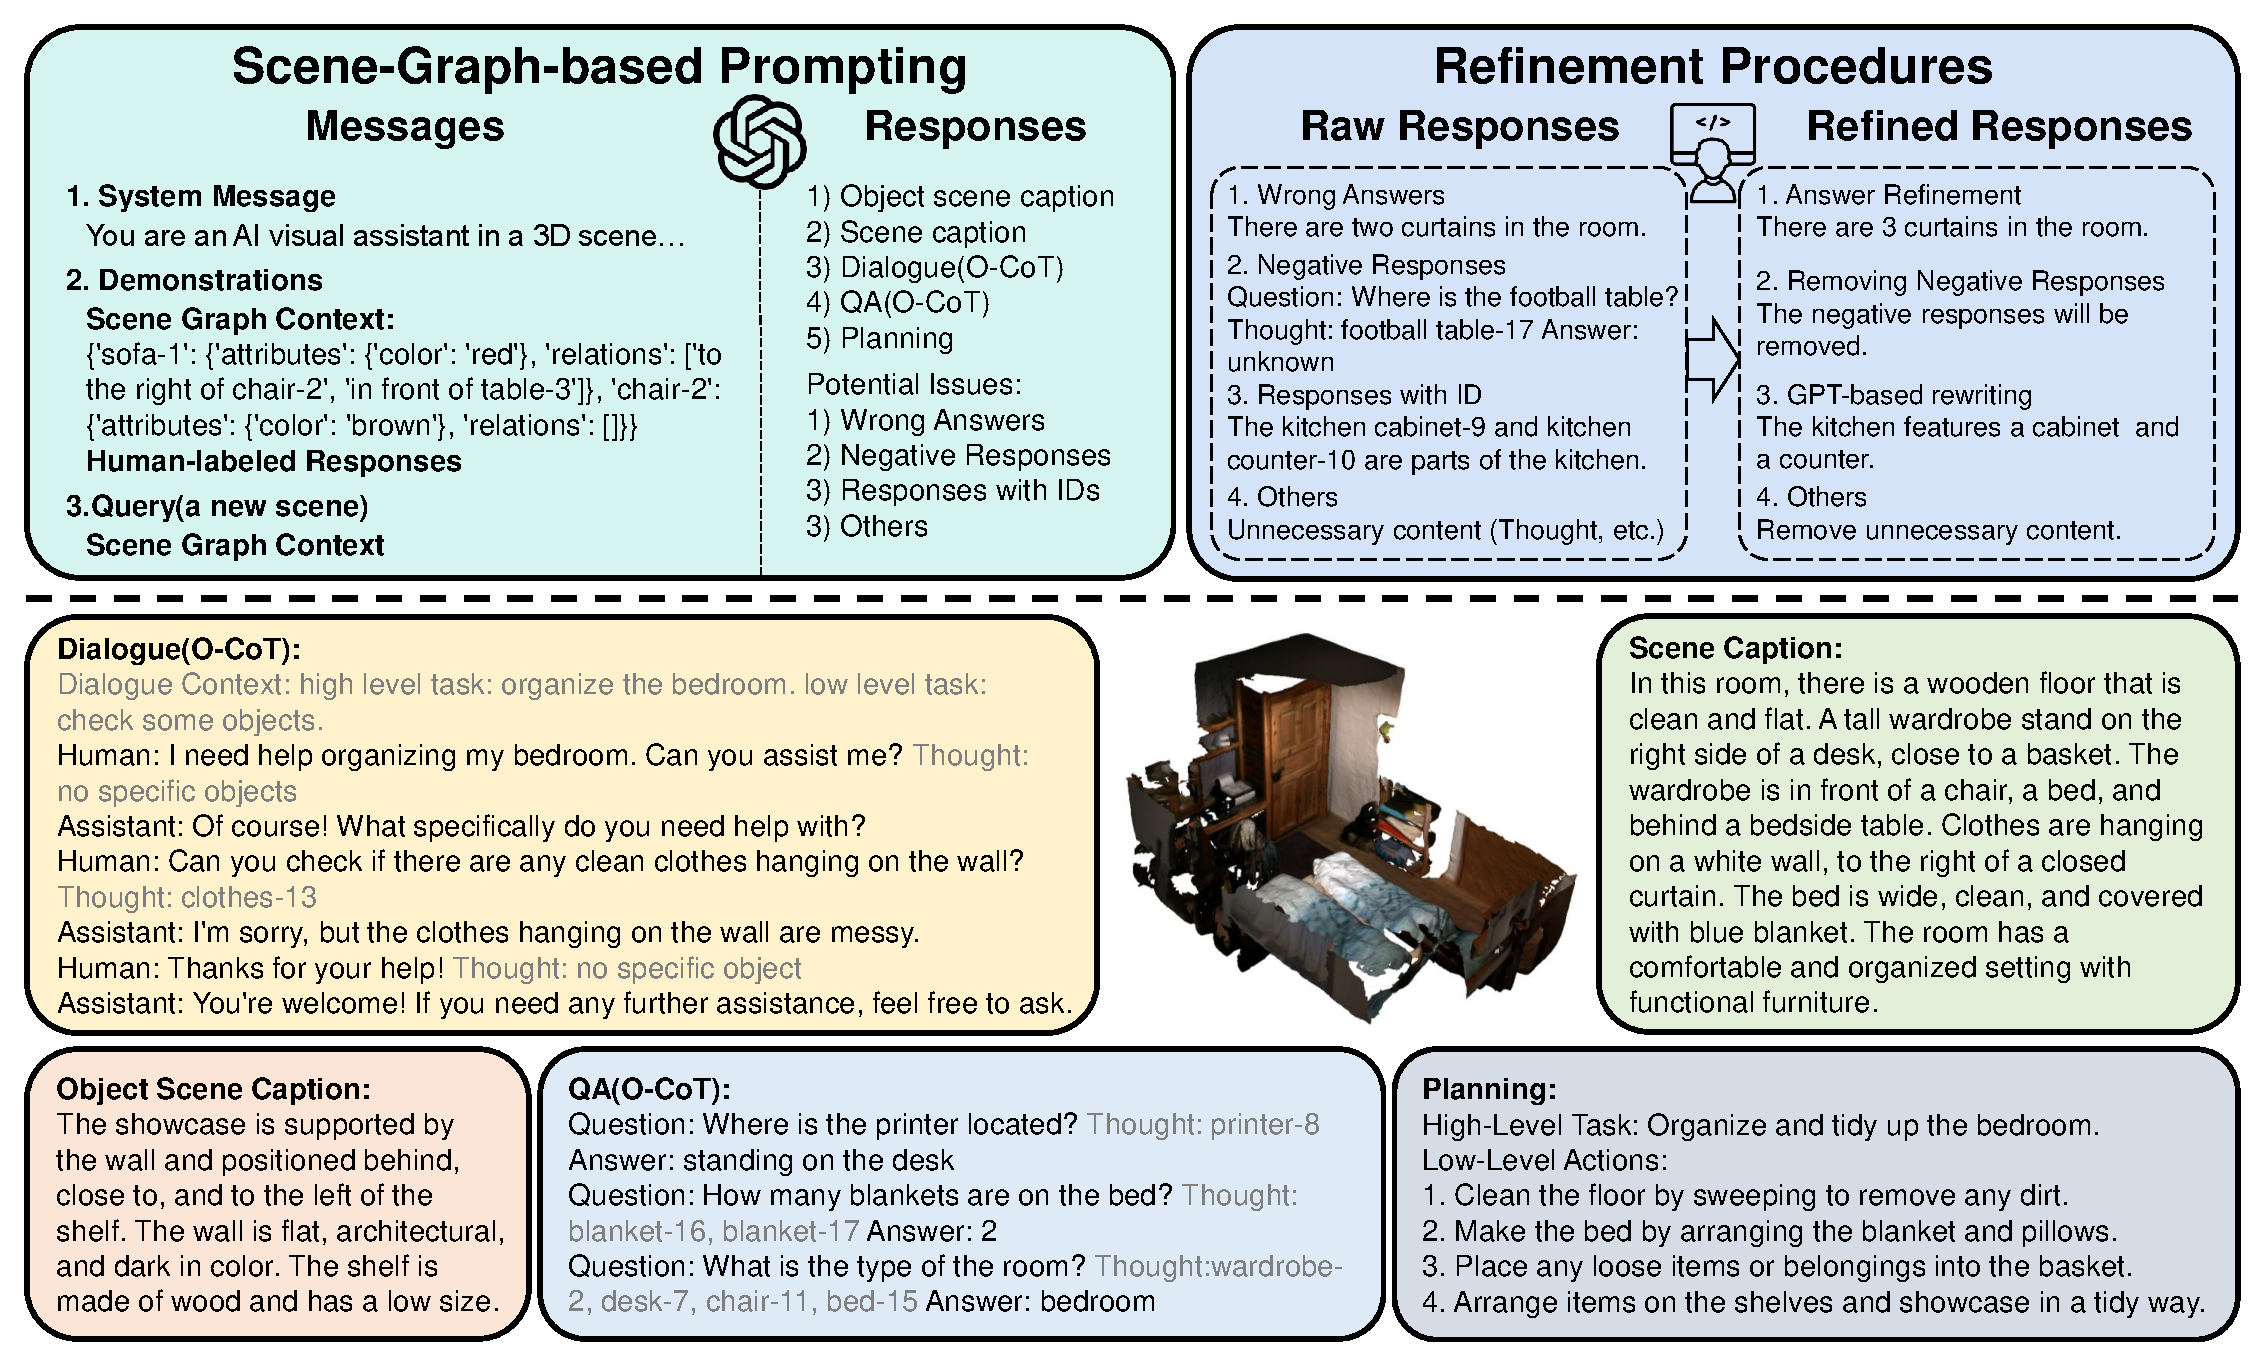
\includegraphics[width=\textwidth, keepaspectratio]{figs/data_framework_0131.pdf}%
  \caption{\textbf{Our proposed LLM-assisted 3D-language data generation pipeline and data examples.}. (Top-left) Messages with 3D scene graphs,
  including object attributes and relations in a phrasal form,
  used for providing scene context when prompting LLM.
  (Top-right) The human-defined refinement procedures were conducted over raw LLM responses to improve data quality.
  (Bottom) Examples of LLM-assisted generation in \agent-align and \agent-instruct. \textcolor{gray}{Thoughts, colored in gray, will be removed after refinements}.}
  \label{fig:data_framework}
  \vskip -0.15in
\end{figure*}

\subsection{\agent-instruct: Instruction Following in 3D world}\label{sec:sft}
In \agent-instruct, \agent will be tuned to follow instructions and accomplish various 3D \ac{vla} tasks. We curate a comprehensive set of tasks that covers a broad spectrum from grounded scene understanding and reasoning~\citep{chen2021scan2cap, ma2023sqa3d}, to dialogue, planning, and embodied acting~\citep{savva2019habitat,cliport}. Specifically, we introduce 1) \textbf{3D captioning and question answering} -- given 3D scene input, the agent needs to generate a natural language response to describe the scene or answer questions; 2) \textbf{3D dialogue and task planning}, where the agent is expected to generate flexible and coherent responses to complex instructions with respect to the given 3D scene, and 3) \textbf{navigation and manipulation}, which require the agent to accomplish a variety of embodied acting tasks in the 3D scene. We defer details to \cref{app:dataset:leo_instruct}.


\subsection{LLM-assisted 3D-language Data Generation}\label{sec:data:generation}
As mentioned above, at the core of producing a large proportion of \agent-align and \agent-instruct is the assistance of LLMs. We now detail the key techniques of prompting LLMs (\ie, ChatGPT) to generate 3D-text paired data. An overview can be found in \cref{fig:data_framework}.

\paragraph{Scene-graph-based prompting.} Our data generation pipeline starts with 3D scene graphs from 3DSSG~\citep{wu2021scenegraphfusion}, which provide scene contexts for prompting. 
Compared to counterparts that utilize object boxes~\citep{yin2023lamm,hong20233d,wang2023chat}, it offers both rich object attributes and accurate spatial relation information among objects, allowing \ac{llm} to generate data with high-quality 3D details (comparisons in \cref{sec:scene graph prompting and bbox prompting}). Next, we manually design some examples as seed tasks~\cite{liu2023visual}, including scene and object captioning, QA, dialogue, and planning, and ask LLM to produce more tasks as well as the responses. Details for designing the seed tasks can be found in~\cref{app:dataset:seed_task}.

\paragraph{Object-centric CoT.} To further combat the \textbf{hallucination} of \ac{llm}~\citep{bang2023hallucination} in open-ended generation as in our pipeline, we propose the object-centric chain of thought (\ac{ocot}) prompting that requires the LLM to explicitly provide the label and ID of object candidates as \textcolor{gray}{thoughts} during text generation. We also utilize subgraph sampling to further enhance the diversity of 3D scene graphs (see details in \cref{app:subgraph_sampling}). We provide examples of \ac{ocot} in~\cref{fig:data_framework}. 















\paragraph{Refinement procedures.} Upon the scene graph and O-CoT prompting, we introduce refinement as an additional safeguard to the quality and reliability of our generated data. Specifically, we send raw LLM responses to several human-defined filters based on the 3D scene graphs: negative responses (\eg, lacking the necessary information to answer) will be removed; unnatural narratives will be rewritten, \etc. Further, we detect text that involves logical reasoning (\eg, counting) or hallucination, and manually fix the wrong responses according to the ground truth provided by scene graphs. We provide illustrative examples in \cref{fig:data_framework} and \cref{app:dataset:refine:examples}, and quantitative analysis on the impact of data refinement procedures in \cref{sec:impact_data_refinement}. %




\paragraph{Assess the quality of generated data.} In addition to data examples, we propose to assess the quality of generated data quantitatively. We focus on the LLM-produced question-answer pairs about objects (questions starting with \textit{How many/Is there} and ending with \textit{in the room/bedroom/kitchen/living room/bathroom}). We first divide these pairs into three categories: \textit{counting}, \textit{existence}, and \textit{non-existence}, which examines the number of certain objects/whether an object exists/whether an object does not exist in the scene, respectively. We manually check if the answers in these pairs are correct, and report the overall accuracy. Results in \cref{tab:data_quality_comparison} demonstrate that our proposed scene-graph-based prompting, O-CoT prompting and refinement bring consistent improvement to data quality and the complete data generation pipeline outperforms a recent counterpart (3D-LLM). We also demonstrate how we help address the \textbf{grammatical errors} compared to counterparts in \cref{app:additional_data_comparison}. Finally, we provide the data distribution in \cref{app:dataset statistics} to illustrate the \textbf{diversity} of our generated data. 











\begin{table*}
\begin{minipage}{0.635\linewidth}
\centering
\captionof{table}{\textbf{Quantitative comparison with \sota models on 3D VL understanding and embodied reasoning tasks}. ``C'' stands for ``CIDEr'', ``B-4'' for ``BLEU-4'', ``M'' for ``METEOR'', ``R'' for ``ROUGE'', ``Sim'' for sentence similarity, and ``EM@1'' for top-1 exact match. The n-gram metrics for Scan2Cap are governed by IoU@0.5. $^\dagger$ indicates answering questions via prompting GPT-3 with the generated scene caption. \textcolor{gray}{Gray} indicates evaluation results with refined exact-match protocol.}
\vspace{0.1em}
\resizebox{\linewidth}{!}{
\begin{tabular}{lccccccccccc}
    \toprule
     & \multicolumn{5}{c}{Scan2Cap (val)} & \multicolumn{5}{c}{ScanQA (val)} & SQA3D (test) \\
     \cmidrule(lr){2-6} \cmidrule(lr){7-11} \cmidrule(lr){12-12}
     & C & B-4 & M & R & Sim & C & B-4 & M & R & EM@1 & EM@1 \\
    \midrule
    \multicolumn{1}{l}{\small\textbf{\textit{Task-specific models}}} \\
    Scan2Cap & 35.2 & 22.4 & 21.4 & 43.5 & - & - & - & - & - & - & \hspace{2pt} 41.0$^\dagger$ \\
    3DJCG & 47.7 & 31.5 & 24.3 & 51.8 & - & - & - & - & - & - & - \\
    Vote2Cap-DETR & 61.8 & 34.5 & 26.2 & 54.4 & - & - & - & - & - & - & - \\
    ScanRefer+MCAN & - & - & - & - & - & 55.4 & 7.9 & 11.5 & 30.0 & 18.6 & - \\
    ClipBERT & - & - & - & - & - & - & - & - & - & - & 43.3 \\
    ScanQA & - & - & - & - & - & 64.9 & 10.1 & 13.1 & 33.3 & 21.1 & 47.2 \\
    \midrule
    \multicolumn{1}{l}{\small\textit{\textbf{Task-specific fine-tuned}}} \\
    3D-VisTA & 66.9 & 34.0 & 27.1 & 54.3 & 53.8 & 69.6 & 10.4 & 13.9 & 35.7 & 22.4 & 48.5 \\
    3D-LLM (FlanT5) & - & - & - & - & - & 69.4 & 12.0 & 14.5 & 35.7 & 20.5 & - \\
    \midrule

    \agent & \textbf{72.4} & \textbf{38.2} & \textbf{27.9} & \textbf{58.1} & \textbf{55.3} & \textbf{101.4} & \textbf{13.2} & \textbf{20.0} & \textbf{49.2} & \textbf{24.5 \textcolor{gray}{(47.6)}} & \textbf{50.0 \textcolor{gray}{(52.4)}} \\
    

    
    
    
    


    \bottomrule
\end{tabular}
}
\label{tab:vl_results}
\end{minipage}
\hfill
\begin{minipage}{0.345\linewidth}
    \vspace{-0.05em}
    \centering   
    \small
    \captionof{table}{\label{tab:test_result_act_cliport} \textbf{Results on robot manipulation}. {\color{mygreen}{seen}} indicates in-domain tasks. {\color{myred}{unseen}} marks OOD tasks with novel colors or objects.}
    \vspace{-0.25em}
    \setlength\tabcolsep{2pt}
    \resizebox{\linewidth}{!}{
    \begin{tabular}{llllccccccccccccccc}
    \toprule
    \multicolumn{4}{l}{} & \multicolumn{4}{c}{\small{separating-piles}} & \multicolumn{4}{c}{\small{\makecell{packing-google\\-objects-seq}}} & \multicolumn{4}{c}{\small{\makecell{put-blocks-in\\-bowls}}} \\
    \cmidrule(lr){5-8}\cmidrule(lr){9-12}\cmidrule(lr){13-16}
    \multicolumn{4}{c}{}& \multicolumn{2}{c}{\color{mygreen}{seen}} & \multicolumn{2}{c}{\color{myred}{unseen}} & \multicolumn{2}{c}{\color{mygreen}{seen}} & \multicolumn{2}{c}{\color{myred}{unseen}} & \multicolumn{2}{c}{\color{mygreen}{seen}} & \multicolumn{2}{c}{\color{myred}{unseen}} \\
    
    \midrule
    
    \multicolumn{4}{l}{CLIP-only}        & \multicolumn{2}{c}{90.2} & \multicolumn{2}{c}{71.0} & \multicolumn{2}{c}{95.8} & \multicolumn{2}{c}{57.8} & \multicolumn{2}{c}{97.7} & \multicolumn{2}{c}{44.5} \\
    
    \multicolumn{4}{l}{CLIPort (single)}          & \multicolumn{2}{c}{98.0} & \multicolumn{2}{c}{\textbf{75.2}} & \multicolumn{2}{c}{\textbf{96.2}} & \multicolumn{2}{c}{71.9} & \multicolumn{2}{c}{\textbf{100}} & \multicolumn{2}{c}{25.0} \\

    \multicolumn{4}{l}{CLIPort (multi)}          & \multicolumn{2}{c}{89.0} & \multicolumn{2}{c}{62.8} & \multicolumn{2}{c}{84.4} & \multicolumn{2}{c}{70.3} & \multicolumn{2}{c}{\textbf{100}} & \multicolumn{2}{c}{\textbf{45.8}} \\
    
    \midrule
    
    \multicolumn{4}{l}{\agent}  & \multicolumn{2}{c}{\textbf{98.8}} & \multicolumn{2}{c}{\textbf{75.2}} & \multicolumn{2}{c}{76.6} & \multicolumn{2}{c}{\textbf{79.8}} & \multicolumn{2}{c}{86.2} & \multicolumn{2}{c}{35.2} \\
    \bottomrule
\end{tabular}
}
    \vfill
\centering
\small
\setlength\tabcolsep{2pt}
\captionof{table}{\label{tab:test_result_act_objnav}\textbf{Results on object navigation.} {$^\dagger$ indicates zero-shot evaluation.}}
\resizebox{\linewidth}{!}{
\begin{tabular}{lcccccc}
\toprule
 \multicolumn{2}{c}{\multirow{2}{*}{}} & \multicolumn{2}{c}{\small{MP3D-val}} & & \multicolumn{2}{c}{\small{HM3D-val}} \\ \cmidrule(lr){3-4}\cmidrule(lr){6-7}
\multicolumn{2}{l}{} &  \small{Success$(\uparrow)$} & \small{SPL$(\uparrow)$} & & \small{Success$(\uparrow)$} &  \small{SPL$(\uparrow)$}\\ \midrule
\multicolumn{2}{c}{Habitat-web (shortest)} & 4.4 & 2.2 & & - &  - \\
\multicolumn{2}{c}{Habitat-web (demo)} & \textbf{35.4} & 10.2 & & - & - \\
\multicolumn{2}{c}{ZSON} & 15.3$^\dagger$ & 4.8$^\dagger$ & & \textbf{25.5} & 12.6 \\
\midrule
\multicolumn{2}{c}{\agent} & 23.1 & \textbf{15.2} & & 23.1$^\dagger$ & \textbf{19.1}$^\dagger$ \\
\bottomrule

\end{tabular}
}  
\end{minipage}
\vskip -0.15in
\end{table*}

\section{Capabilities and Analyses}\label{sec:exp}
We demonstrate \agent's capabilities by a comprehensive evaluation on the full spectrum of embodied 3D tasks encompassing perceiving, grounding, reasoning, planning, and acting.
In \cref{sec:exp_3dvl}, we present quantitative comparisons between \agent and \sota models on various 3D VL tasks, underscoring \agent's proficiency in 3D VL understanding and reasoning. In \cref{sec:exp_dialog}, we highlight \agent's strength in scene-grounded dialogue and task planning. In \cref{sec:exp_eai}, we extend \agent to embodied acting tasks wherein \agent exhibits remarkable versatility. In \cref{sec:ablation}, we conduct ablative studies to reveal more insights into \agent, including data and model aspects. In \cref{sec:exp_scaling}, we probe the scaling effect and manifest the potential for further development.


\subsection{3D Vision-Language Understanding and Reasoning}\label{sec:exp_3dvl}

\paragraph{Overview.} Understanding and reasoning about object attributes, object relations, and other facets of 3D scenes from an agent's egocentric perspective is a fundamental capability of an embodied generalist agent in the 3D world. We investigate \textit{how well can \agent perform 3D VL understanding and embodied reasoning tasks, especially when being compared against task-specific models and existing generalist agents}. Specifically, we consider three renowned 3D tasks: 3D captioning on Scan2Cap~\citep{chen2021scan2cap}, 3D QA on ScanQA~\citep{azuma2022scanqa}, and 3D embodied reasoning on SQA3D~\citep{ma2023sqa3d}. Our evaluation metrics include conventional scores (\eg, CIDEr, BLEU, METEOR, ROUGE) and other metrics adapted for open-ended generation, \eg, sentence similarity \citep{reimers2019sentence} and refined exact-match accuracy (see details in \cref{sec:supp_eval_qa}).
Following 3D-VisTA~\citep{zhu20233d}, \textbf{we use object proposals from Mask3D~\citep{schult2022mask3d} instead of ground-truth object segments for evaluation.}


\paragraph{Baselines.} For quantitative comparisons, we include both task-specific approaches and generalist models: 1) \sota specialists in 3D dense captioning \citep{chen2021scan2cap,cai20223djcg,chen2023end}; 2) \sota specialists in 3D QA \citep{azuma2022scanqa,ma2023sqa3d}; 3) task-specific fine-tuned generalist models like 3D-VisTA \citep{zhu20233d} and 3D-LLM \citep{hong20233d}. To the best of our knowledge, \textit{\agent is the first model that, in stark contrast to prior models, can directly handle the aforementioned 3D VL tasks in a unified architecture without task-specific fine-tuning}. This lends greater credence to \agent's comparative superiority.




    

    
    
    
    



    
    
    

    
    



\paragraph{Results \& analysis.} As shown in \cref{tab:vl_results}, \agent surpasses both \sota single-task and task-specific fine-tuned models significantly on 3D dense captioning and 3D QA tasks. In contrast to the specialist models that utilize task-specific heads, our LLM-based approach not only affords the flexibility of generating open-ended responses but also exhibits excellent quantitative results. On the other hand, considering the complicated feature aggregation in 3D-LLM, we believe that object-centric 3D representation is a simple yet effective option to connect 3D scenes with LLM while harnessing the inherent knowledge of LLM.

\vspace{-0.3em}
\subsection{Scene-grounded Dialogue and Planning}\label{sec:exp_dialog}

\paragraph{Overview.} Upon the 3D VL understanding and reasoning, we anticipate \agent to support more sophisticated interaction with humans, \eg, responding to complex multi-round user instructions in the 3D world. To verify these capabilities, we conduct qualitative studies on 3D dialogue and planning tasks, with unseen scenarios from the held-out test sets of \agent-instruct. We defer the quantitative results of dialogue and planning to our ablation study in \cref{sec:ablation}. Quantitative comparison with other approaches is infeasible given the absence of comparable benchmarks.

\paragraph{Results \& analysis.} As shown in \cref{fig:qualitative}, \agent is capable of generating high-quality responses, which encompass two features: \textbf{1) Precisely grounded to the 3D scenes.} The task plan proposed by \agent involves concrete objects related to the 3D scene, as well as plausible actions regarding these objects. \textbf{2) Rich informative spatial relations.} The entities in \agent's responses often accompany detailed depictions. Such information helps identify specific objects in complex 3D scenes and affords considerable assistance to humans.

\begin{table*}
\begin{minipage}{0.41\linewidth}
    \centering
    \captionof{table}{Quantitative results of \agent trained with different data configurations. \textit{w/o Align}: without alignment stage. \textit{ScanNet}: tuned on ScanNet scenes only. \textit{w/o Act}: tuned without embodied acting tasks. We report the exact match metrics for QA tasks and sentence similarity for others. \underline{Underlined figures} indicate zero-shot results on novel scenes (3RScan).}
    \setlength\tabcolsep{3pt}
    \resizebox{\linewidth}{!}{
    \begin{tabular}{lcccccc}
        \toprule
     & \multicolumn{3}{c}{ScanNet} & \multicolumn{3}{c}{3RScan} \\
     \cmidrule(lr){2-4} \cmidrule(lr){5-7}
         & Scan2Cap & ScanQA & SQA3D & 3RQA & 3RDialog & 3RPlan \\
        \midrule
        \rowcolor{color1} \textit{w/o Align} & 62.8 & 22.7 \textcolor{gray}{(45.0)} & \textbf{50.9 \textcolor{gray}{(53.2)}} & 49.7 \textcolor{gray}{(53.7)} & 73.0 & 80.3 \\
        \rowcolor{color2} \textit{ScanNet} & 64.0 & 24.4 \textbf{\textcolor{gray}{(49.2)}} & 46.8 \textcolor{gray}{(49.5)} & \underline{35.8 \textcolor{gray}{(50.0)}} & \underline{25.5} & \underline{23.4} \\
        \textit{w/o Act} & \textbf{65.4} & 24.3 \textcolor{gray}{(48.5)} & 50.0 \textcolor{gray}{(52.5)} & \textbf{51.9 \textcolor{gray}{(57.4)}} & \textbf{73.3} & \textbf{81.1} \\
        \rowcolor{color4} \textit{VLA} & 65.3 & \textbf{25.0} \textcolor{gray}{(48.9)} & 46.2 \textcolor{gray}{(48.3)} & 51.3 \textcolor{gray}{(55.8)} & 72.3 & 77.2 \\
        \bottomrule
    \end{tabular}
    }
    \label{tab:data_ablation}
\end{minipage}
\hfill
\begin{minipage}{0.31\linewidth}
\centering
\small
\setlength\tabcolsep{3pt}
\captionof{table}{TrueSkill scores with human preference. \textit{Dialg}: dialogue and planning data.}\label{tab:response_trueskill}
    \resizebox{\linewidth}{!}{
\begin{tabular}{lccc}
\toprule
 & Answerable & Unanswerable & NLP \\
 \midrule
 \textit{w/o Dialg} & 24.4$\pm$1.3 & 23.1$\pm$1.4  & 23.4$\pm$1.4 \\
 \textit{w/ Dialg} & \textbf{25.6}$\pm$\textbf{1.3}  & \textbf{26.8}$\pm$\textbf{1.4} & \textbf{26.6}$\pm$\textbf{1.4} \\
 \bottomrule 
\end{tabular}
}
\vfill
\vspace{0.3em}
\centering
\small
\captionof{table}{Answer accuracy (EM) on object-existence questions. \textit{Aug}: augmented data.}\label{tab:data_balance}
\resizebox{\linewidth}{!}{
\begin{tabular}{lcccccccc}
    \toprule
     & \multicolumn{3}{c}{3RScan} & \multicolumn{3}{c}{ScanNet (0-shot)} \\
     \cmidrule(lr){2-4} \cmidrule(lr){5-7}
     & Yes & No & Overall & Yes & No & Overall \\
     \midrule
    \textit{w/o Aug} & \textbf{1.00} & 0.01 & 0.34 & \textbf{0.98} & 0.16 & 0.43 \\
    \textit{w/ Aug} & 0.72 & \textbf{0.91} & \textbf{0.85} & 0.88 & \textbf{0.81} & \textbf{0.83} \\
    \bottomrule
\end{tabular}
}
\end{minipage}
\hfill
\begin{minipage}{0.263\linewidth}
    \centering
    \captionof{figure}{\label{fig:scaling_law}\agent-instruct test loss with the growth of data and model scale, manifesting the scaling law.}
    \vspace{0.2em}
    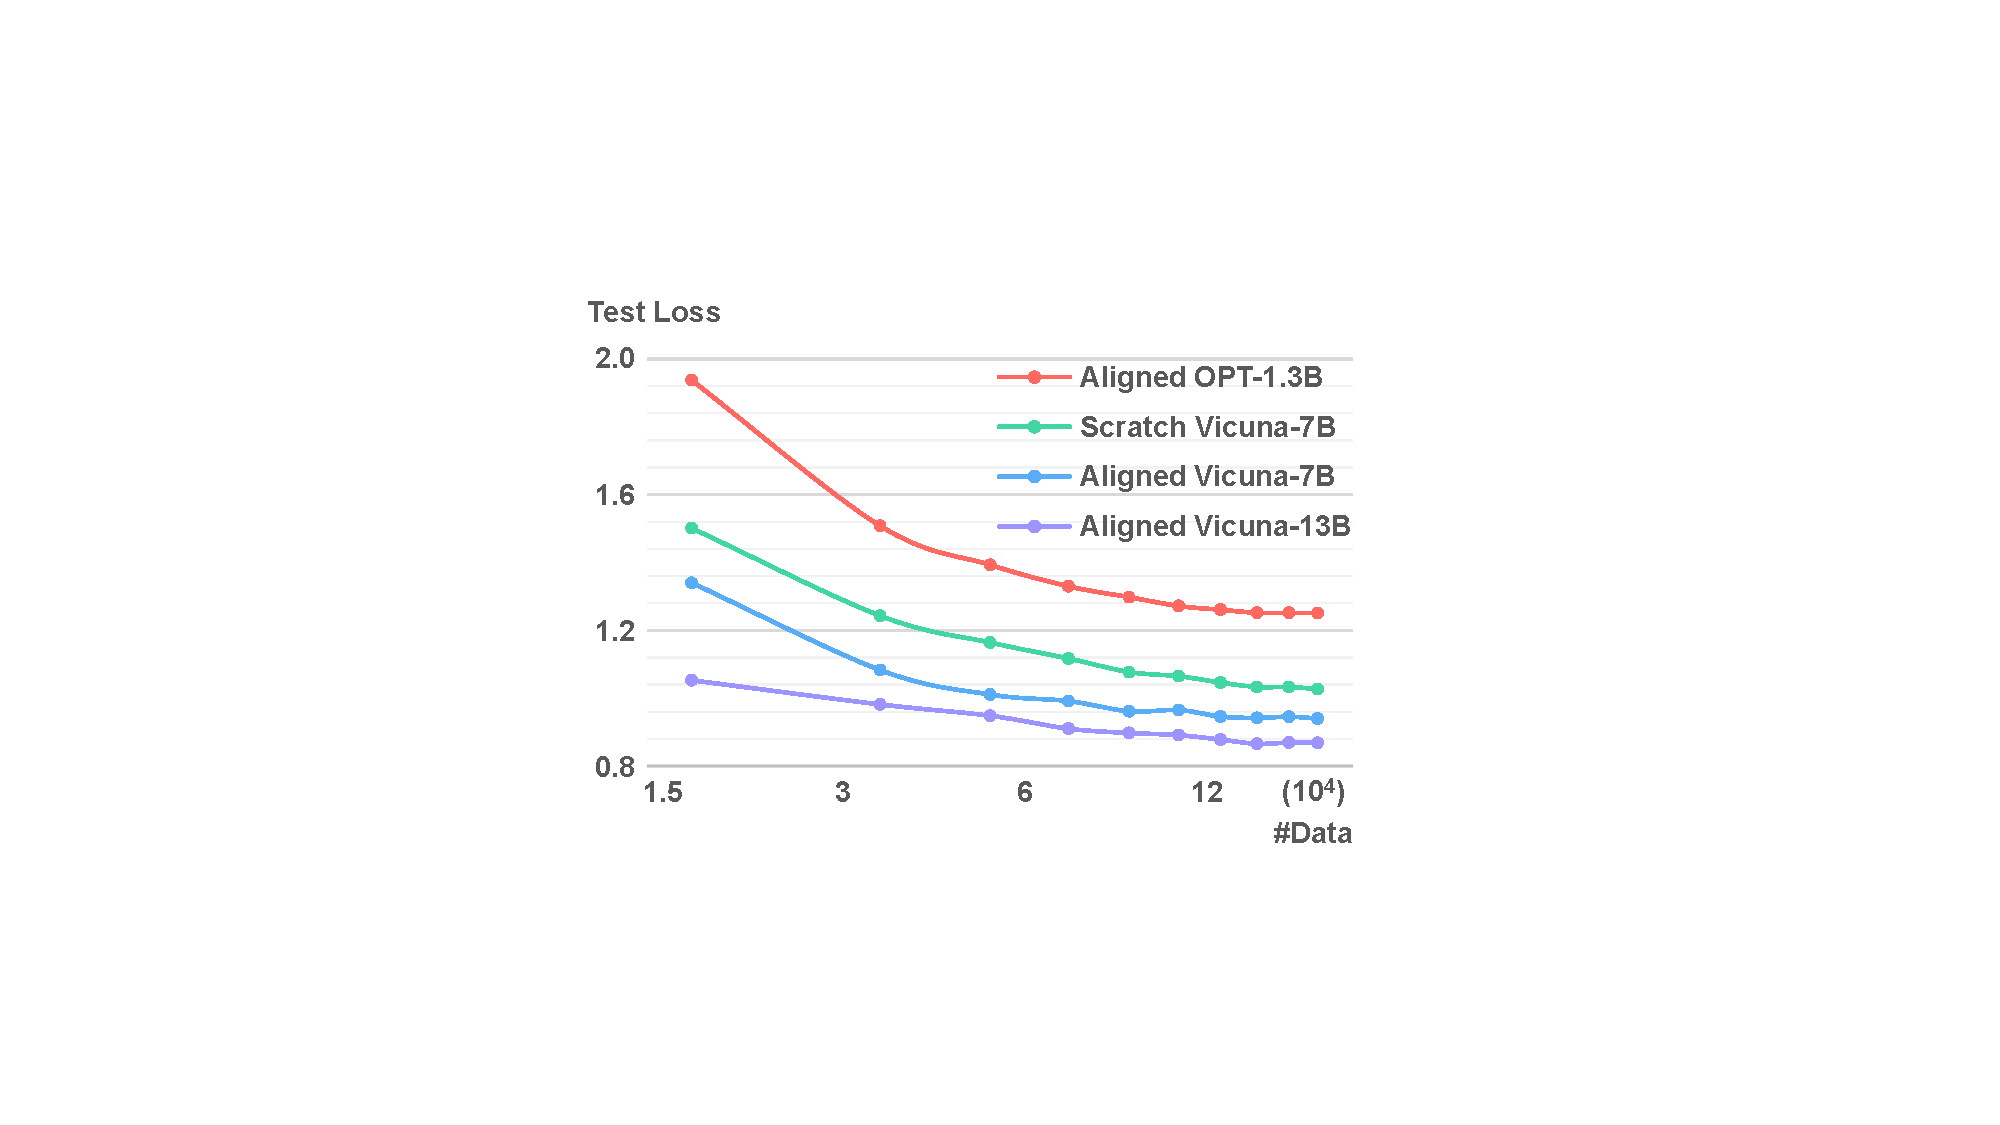
\includegraphics[width=\linewidth]{figs/scaling_law.pdf}
\end{minipage}
\end{table*}


\subsection{Embodied Action in 3D World}\label{sec:exp_eai}

\paragraph{Overview.} To probe \agent's capacity of bridging vision-language-acting in the 3D world, we select two canonical embodied AI tasks: embodied navigation (\texttt{ObjNav}) on AI Habitat~\citep{ramrakhya2022habitat} and robotic manipulation on CLIPort~\citep{cliport}.
Specifically, for CLIPort robotic manipulation, we evaluate \agent on the three tasks listed in~\cref{tab:test_result_act_cliport} including their unseen counterparts, and report the success scores. For \texttt{ObjNav}, 
we evaluate \agent on the original MP3D \texttt{ObjNav} validation split. Additionally, we test generalization to the validation split of the newly introduced HM3D \texttt{ObjNav} task~\citep{ramakrishnan2021habitat}. We report the success rate and SPL metrics following \citet{ramrakhya2022habitat}. We consider both Habitat-web \citep{ramrakhya2022habitat} (fully supervised) and ZSON \citep{majumdar2022zson} (zero-shot) as baselines.

\paragraph{Results \& analysis.} We present the results of CLIPort manipulation and object navigation in~\cref{tab:test_result_act_cliport,tab:test_result_act_objnav}. Our findings are as follows: 1) In robotic manipulation, \agent is comparable to \sota performances and even better on some challenging {\color{myred}{unseen}} tasks. In particular, \agent directly produces motor commands without inductive bias (\eg, heatmap) that benefit previous methods, showcasing \agent's considerable capacity for learning embodied actions. 2) In \texttt{ObjNav}, \agent achieves a success rate that is comparable to the baselines and has a better SPL on MP3D-val, suggesting that \agent can leverage the object-centric 3D scene input (potentially offering a coarse global map) and take a shorter path to the target. Furthermore, results on HM3D-val confirm \agent's zero-shot generalization to novel scenes. Notably, all baselines are equipped with recurrent modules while \agent only incorporates truncated past actions, which could account for a lower success rate (see discussion in \cref{sec:supp_eai_split}). 3) Overall, the two-stage learning scheme endows \agent with semantic-level generalization (novel objects, \etc) in both manipulation and navigation tasks. We demonstrate the efficacy of tackling embodied acting tasks with a general framework from 3D VL.

\paragraph{Additional results.} We further investigate the perception modules, data regime, and generalization to unseen objects in \texttt{ObjNav} task. See the results in \cref{sec:result_objnav_additional}.



\vskip -0.15in
\subsection{More Insights into \agent}\label{sec:ablation}

\paragraph{Overview.} In this section, we aim to offer deeper insights into \agent's characteristics, mainly from the data perspective (model perspective is deferred to \cref{sec:model_ablation}). Specifically, we evaluate \agent when trained with different data configurations, including exact match, sentence similarity, and human rating. We regard \agent instruction-tuned without embodied acting tasks (\textit{w/o Act}) as the default setting. Following \citet{achlioptas2020referit3d}, we use ground-truth object segments in these analyses. We present additional analyses on data in \cref{sec:data_comparison} and model in \cref{sec:model_comparison}.

\paragraph{Alignment stage.} In contrast to complete two-stage training (\textit{w/o Act}), we direct instruction-tune a model without alignment stage (\textit{w/o Align}). The results in \cref{tab:data_ablation} show the consistent impact of alignment. In particular, the benefit of alignment is significant on Scan2Cap since it concerns detailed scene understanding and captioning, which is a primary focus of alignment training. %

\paragraph{Specialist \vs generalist.} We train a specialist on ScanNet scenes (\textit{ScanNet}). As shown in \cref{tab:data_ablation}, \textit{ScanNet} performs slightly worse than \textit{w/o Act} even on ScanNet tasks, and particularly struggles at generalization across scenes (3RQA) and tasks (3RDialog and 3RPlan). This demonstrates the advantage of generalist-style instruction tuning with broad coverage of scenes and tasks.

\paragraph{VL \vs VLA.} We compare \textit{w/o Act} and \textit{VLA}, which differ in whether embodied acting tasks are included for training. The results in \cref{tab:data_ablation} show that incorporating embodied acting tasks could lead to performance drops on 3D VL tasks. This may stem from 1) the gap between language generation and embodied action prediction, and 2) the imbalanced data scale of embodied acting tasks. In contrast to the finding that VL data benefits embodied acting tasks in VLA co-training \citep{brohan2023rt}, our observation implies that embodied acting tasks may harm VL capabilities in turn. How to continually bridge the gap between VL and embodied acting tasks is an important direction for further exploration.


\paragraph{Dialogue and planning data.} In contrast to the default model (\textit{w/ Dialg} in \cref{tab:response_trueskill}), we train \agent without dialogue and planning data (\textit{w/o Dialg}). We design an evaluation set with three types of questions (Answerable, Unanswerable, and NLP) and evaluate with TrueSkill~\citep{graepel2007bayesian} according to human preference (see details in \cref{sec:dialog_planning}). The results in \cref{tab:response_trueskill} confirm more hallucinations (less preferred by users on ``Unanswerable'') and worse NLP skills for \textit{w/o Dialg}. This is probably because 1) the diverse conversations in our dialogue data can help cultivate flexible responses to complex instructions, and 2) our planning data can offer scene-grounded commonsense knowledge and also encourage detailed coherent text.



\paragraph{Data balancing.} We find imbalanced data could induce hallucination in \agent, \eg, it tends to respond with ``Yes'' when asked ``Is there something in this room?''. To address this, we augment the 3RScanQA data with more negative samples where non-existent objects are queried. We also design an evaluation set with different types (Yes and No) of object-existence questions (see details in \cref{sec:data_balancing}). Results in \cref{tab:data_balance} demonstrate that we can effectively mitigate the hallucination problem by balancing the tuning data. Moreover, the benefit of augmenting 3RScan data can transfer to ScanNet scenes in a zero-shot manner.









\subsection{Scaling Law Analysis}\label{sec:exp_scaling}

\paragraph{Settings.} 
We study the scaling effect~\citep{kaplan2020scaling,reed2022generalist} of data and model in \agent by tracking the instruction-tuning loss on the test set with the growth of data scale. In addition to the default Vicuna-7B, we incorporate two LLMs at different scales: OPT-1.3B \citep{zhang2022opt} and Vicuna-13B \citep{vicuna2023}. For Vicuna-7B, we also probe the influence of alignment (Scratch \vs Aligned).


\paragraph{Results \& analysis.} From the test loss curves in \cref{fig:scaling_law}, we have the following findings: \textbf{1) The instruction tuning of \agent conforms to the scaling law}~\citep{kaplan2020scaling,reed2022generalist}. We observe that all curves decrease log-linearly with the data scale. \textbf{2) Scaling up LLM leads to consistent improvements.} Aligned Vicuna-7B shows significantly lower losses than Aligned OPT-1.3B. In contrast, despite the consistent improvements, the gap between Aligned Vicuna-7B and Vicuna-13B appears less significant, suggesting potential saturation if we continue to scale up the LLM. This indicates the scalability of \agent and the necessity of scaling up data to match the model capacity. \textbf{3) Alignment leads to consistent improvements.} Aligned Vicuna-7B shows consistently lower losses than Scratch Vicuna-7B, which corresponds to the inferior performances of \textit{w/o Align} in \cref{tab:data_ablation}.














    
    
    
    





\paragraph{Search with LLM}
Effective search strategy has been shown crucial for tasks that involve complex reasoning and planning, such as go \citep{silver2016mastering} and math reasoning \citep{gsm8k,math}.
For math reasoning tasks, various search methods have been studied.
One direction of research \citep{zhu2024deductive,xie2024self} designed beam search with dynamic pruning, where beam items of low quality are pruned.
Another line of work \citep{yao2024tree,long2023large,besta2024graph,hao2023reasoning,feng2023alphazero} maintains a tree or a graph that represents the current progress of solving the input question where potential branches are iteratively expanded.
Both our approach and \cite{feng2023alphazero} are based on the MCTS algorithm, while one main difference is how to define a search step: \cite{feng2023alphazero} fix a search step to be either a token or a sentence, while our approach is more flexible on deciding steps.
We have also carefully designed the MCTS process, incorporating multiple critique signals to guide the search more effectively and introducing adaptive search parameters for improved state exploration.
As the result, our approach achieves much better performances.

\paragraph{LLM Self-improving}
Being a key to the success of scalable oversight \citep{bowman2022measuring},
self-improving for LLM aims to align the LLM to human preference and values mainly using the supervision from the knowledge inside the LLM \citep{zelikman2022star,zelikman2024quiet}.
One crucial part of self-improving is how to obtain reliable signal of critique to distinguish between good responses from the LLM and bad ones.
Initial work \citep{bai2022constitutional,wang2022self} first asks the LLM to generate input queries of diverse tasks and the corresponding outputs.
They then rely on hand-crafted heuristic rules to filter out redundant or low-quality data pairs (e.g. the query is too long or too short). 
Since it is non-trivial to compose effective heuristic rule, later work \citep{sun2023principle,li2023self,guo2024human} proposes a few general principles or judging criteria and ask the LLM itself to evaluate the quality its responses based on these guidance, hoping that LLMs can automatically designate these principles into each data point to better guide data filtering. However, this requires LLMs to have strong abilities to apply these principles for each specific case and make correct judgements. Different from previous work, we propose to leverage the supervision from MCTS for LLM self-improvement: taking the outputs of MCTS to continue train the LLM. This is because the outputs from MCTS are usually in much better quality then standard nucleus sampling, and the large gap ensure that the LLM can self improve.

% Another line of research explores cheaply available knowledge.
% Some \citep{saunders2022self,wang2023shepherd} collects large-scale critique data from question-and-answer websites (e.g., stack exchange) for continue pretraining, while others \citep{gou2023critic} utilize external tools to provide more fine-grained guidance.
% The goal of both directions is to enhance critique ability of the LLM for self-improving.
% Our approach based on MCTS is intuitively orthogonal to this line of research.

\section{Conclusions}\label{sec:conclusion}
The proposed agent \agent extends the current generalist ability of \ac{llm} from text towards the 3D world and embodied tasks. It is a crucial initial step towards building embodied generalist agents. Nonetheless, there are also limitations, \eg, generalization to novel scenes, and a notable gap between VL learning and embodied action control. In light of this work, we identify several promising directions that hold the potential for substantial advancement: (1) enhancing the 3D \ac{vl} understanding capability by leveraging larger-scale VL data from richer 3D domains; (2) continually bridging the gap between 3D \ac{vl} and embodied action, as our experiments reveal the efficacy of their joint learning; (3) investigating the issues of safety and alignment in the context of embodied generalist agents, particularly given that our scaling law analysis suggests significant enhancements through scaling on data and model.

\section*{Impact Statement}
This work introduces LEO, an embodied multi-modal generalist agent designed to extend machine learning capabilities into the 3D realm, marking a significant advance in the field. The potential societal implications of LEO are manifold, touching on robotics, AR/VR, assistive technologies, and environmental planning. Ethically, it underscores the importance of responsible AI development, emphasizing safety, privacy, and fairness in automated decision-making. As LEO ventures into new territories of human-machine interaction, it prompts a re-evaluation of ethical frameworks to ensure that advancement contributes positively to society. While the immediate societal consequences of our work align with the goals of advancing machine learning, we acknowledge the necessity of ongoing ethical consideration as applications of LEO evolve.


\section*{Acknowledgements}
This work is supported in part by the National Science and Technology Major Project (2022ZD0114900).


\bibliography{ref}
\bibliographystyle{icml2024}

\clearpage
\onecolumn
\appendix
\section{Partial Zipping}\label{ap:partial_zipping}
In Fig.~\ref{fig:varying_partial_zip} we plot the average per task accuracy by the number of layers zipped in ResNet-20$\times$8 for CIFAR-100 (50+50) and ResNet-50 for ImageNet-1k (200+200). 
Note that to avoid adding extra unmerge modules into the network, our stopping point while unzipping has to be the end of a stage. 

In Table~\ref{tab:partialzip_corrs}, we show the average neuron correlations at each partial-zipping stage between the layers of ResNet-20 ($8\times$) models trained on the CIFAR-100 (50+50) task. 
We collect results using the same models used in Table \ref{tab:cifar50+50}, and compute correlations as described in Section \ref{sec:approach}.
Overall, we find the correlations between models consistently decreases through successive partial zipping locations. 
This corroborates the finding of \citet{kornblith2019similarity} that model layers become increasingly dissimilar with depth, as they encode more task-specific features. 
Coupling Table \ref{tab:partialzip_corrs} with Figure \ref{fig:partial_zip_cifar100}, we observe a direct correlation between layer-(dis)similarities and performance decrease.
This illustrates the importance of layer similarity between two networks and strong performance.
% \begin{figure}[t]
% \centering

% \subfloat[
%     \textbf{CIFAR-100 50+50.}
%     \label{fig:partial_zip_cifar100}
% ]{
% \centering
% \begin{minipage}{0.49\linewidth}{
% \begin{center}
%     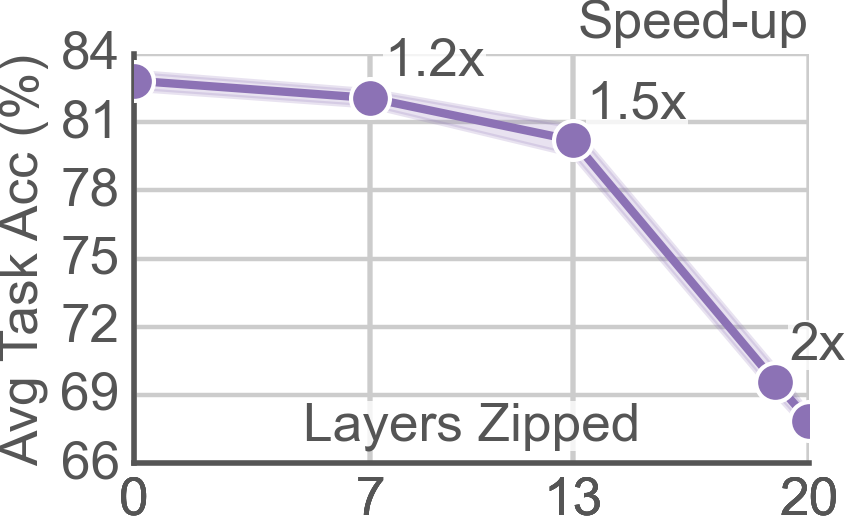
\includegraphics[width=\linewidth]{figures/imgs/partial_zip_CIFAR_50_50.png}
% \end{center}
% }\end{minipage}
% }
% \subfloat[
%     \textbf{ImageNet-1k 200+200.}
%     \label{fig:partial_zip_imagenet}
% ]{
% \centering
% \begin{minipage}{0.49\linewidth}{
% \begin{center}
%     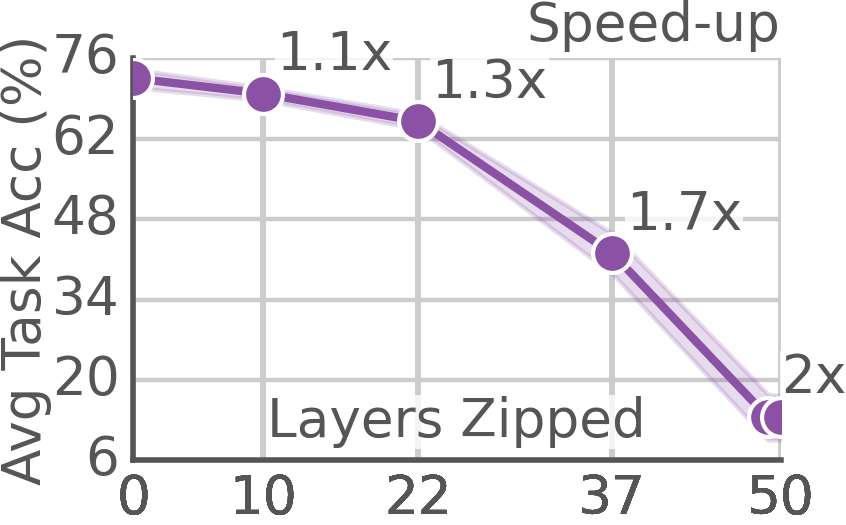
\includegraphics[width=\linewidth]{figures/imgs/partial_zip_imnet_200_200.png}
% \end{center}
% }\end{minipage}
% }

% \caption{
% {\bf Varying Partial Zip.} 
% By leaving some layers unzipped (Sec.~\ref{sec:partial_zip}), we can recover a significant amount of performance while still merging most of the model. 
% }
% \label{fig:varying_partial_zip}
% \end{figure}

% \begin{wrapfigure}{r}{0.48\linewidth}
% \vspace{-10pt}
% \centering
% \resizebox{\linewidth}{!}{
%     \tablestyle{5pt}{1.1}
%     {
%     \tablestyle{5pt}{1.1}
%     \begin{tabular}{x{40}x{40}x{40}}
%         \multicolumn{3}{c}{Average Stage Correlations}\\
%         Layer \sfrac{7}{20} & Layer \sfrac{13}{20} & Layer \sfrac{19}{20}\\
%     \shline
%     {0.50\conf{0.01}} & {0.37\conf{0.00}} & {0.27\conf{0.00}} \\
%     \hline
% \end{tabular}
%     }
% }
% \captionof{table}{\textbf{CIFAR-100 (50+50) Zipping Correlations.} We show the average correlations between two ResNet-20 ($8\times$) models at each partial zipping stage. Correlations consistently decrease at each successive stage, indicating that the layers of the two models increasingly diverge. 
% }
% \label{tab:partialzip_corrs}
% % \end{table}
% \vspace{-20pt}
% \end{wrapfigure}


\begin{wrapfigure}{r}{0.48\linewidth}
\vspace{-15pt}
\begin{minipage}[l]{\linewidth}{
\captionsetup{justification=centering}
\subfloat[
    \textbf{CIFAR-100 \\ \ \ \ \ (50+50)}
    \label{fig:partial_zip_cifar100}
]{
\centering
\begin{minipage}{0.48\linewidth}{
\begin{center}
    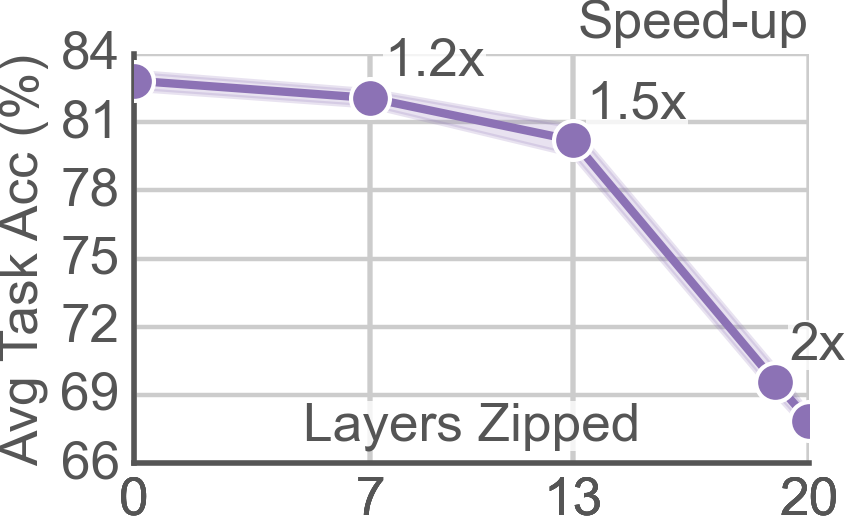
\includegraphics[width=\linewidth]{figures/imgs/partial_zip_CIFAR_50_50.png}
\end{center}
}\end{minipage}
}
\subfloat[
    \textbf{ImageNet-1k \\ \ \ \  (200+200)}
    \label{fig:partial_zip_imagenet}
]{
\centering
\begin{minipage}{0.48\linewidth}{
\begin{center}
    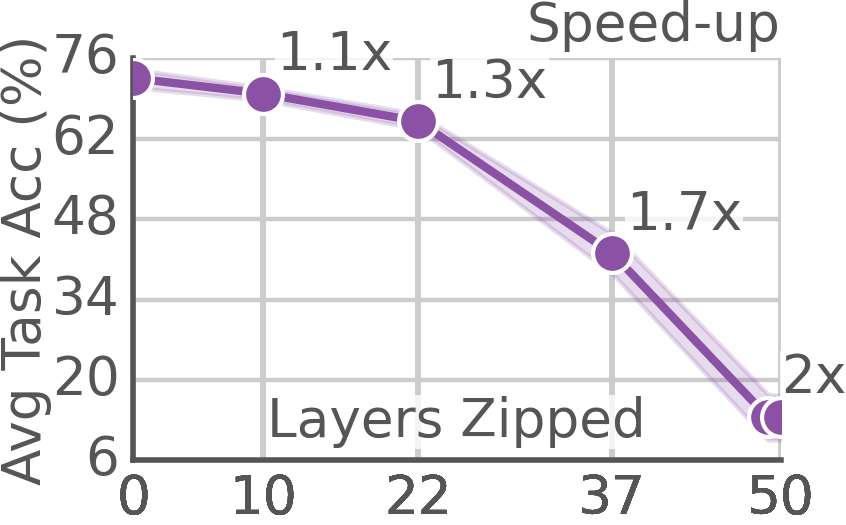
\includegraphics[width=\linewidth]{figures/imgs/partial_zip_imnet_200_200.png}
\end{center}
}\end{minipage}
}
\captionsetup{justification=justified}
        \caption{{\bf Varying Partial Zip.} By leaving some layers unzipped (Sec.~\ref{sec:partial_zip}), we can recover a significant amount of performance while still merging most of the model. }
\label{fig:varying_partial_zip}
}\end{minipage}
\begin{minipage}[l]{\linewidth}{
\vspace{5pt}
\centering
\resizebox{\linewidth}{!}{
    \tablestyle{5pt}{1.1}
    {
    \tablestyle{5pt}{1.1}
    \begin{tabular}{x{40}x{40}x{40}}
        \multicolumn{3}{c}{Average Stage Correlations}\\
        Layer \sfrac{7}{20} & Layer \sfrac{13}{20} & Layer \sfrac{19}{20}\\
    \shline
    {0.50\conf{0.01}} & {0.37\conf{0.00}} & {0.27\conf{0.00}} \\
    \hline
\end{tabular}
    }
}
\captionof{table}{\textbf{CIFAR-100 (50+50) Zipping Correlations.} We show the average correlations between two ResNet-20 ($8\times$ width) models at each partial zipping stage. Correlations consistently decrease at each successive stage, indicating that the layers of the two models increasingly diverge. 
}
\label{tab:partialzip_corrs}
% \end{table}
% \vspace{10pt}
}\end{minipage}
\begin{minipage}[l]{\linewidth}{
\captionsetup{justification=centering}
\vspace{1em}
\subfloat[
    \textbf{CIFAR-100 \\ \ \ \ \ (50+50)}
    \label{fig:data_use_cifar100}
]{
\centering
\begin{minipage}{0.48\linewidth}{
\begin{center}
    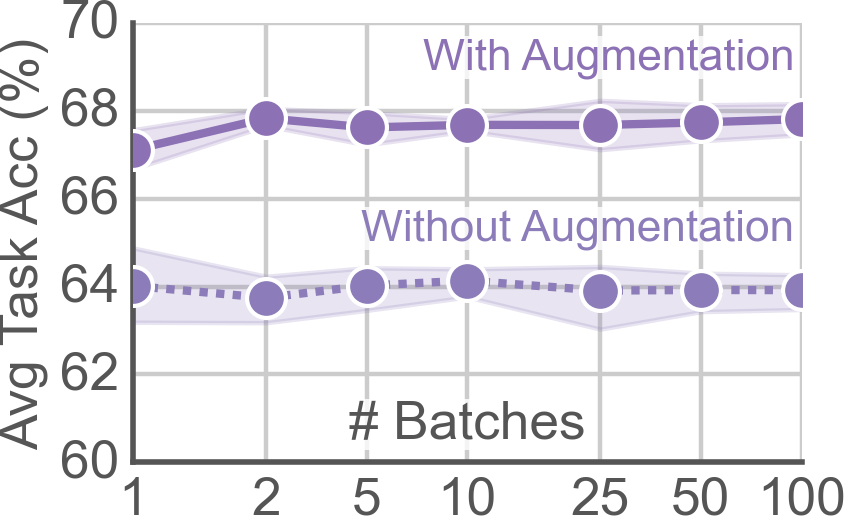
\includegraphics[width=\linewidth]{figures/imgs/cifar100_data.png}
\end{center}
}\end{minipage}
}
\subfloat[
    \textbf{ImageNet-1k \\ \ \ \  (200+200)}
    \label{fig:data_use_imagenet}
]{
\centering
\begin{minipage}{0.48\linewidth}{
\begin{center}
    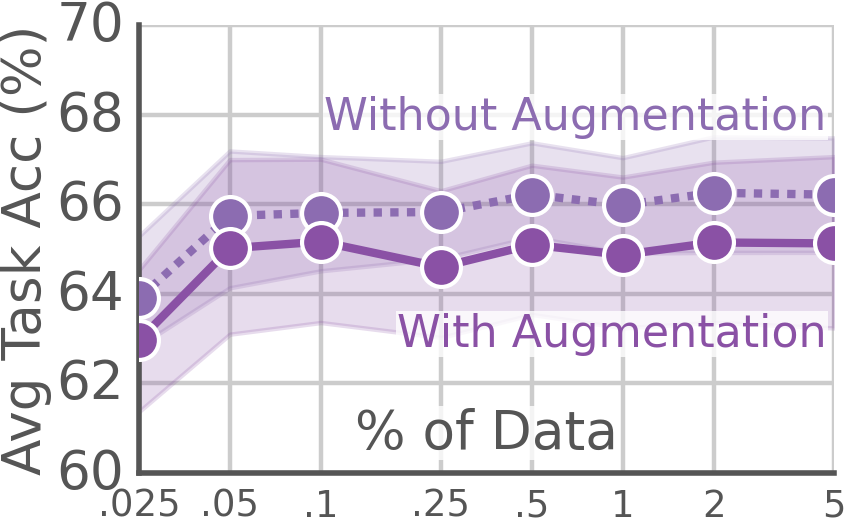
\includegraphics[width=\linewidth]{figures/imgs/imnet200_data.png}
\end{center}
}\end{minipage}
}
\captionsetup{justification=justified}
\caption{
{\bf Data Usage.} 
How much data do we need to use to compute activations? 
We find that only a few hundred images are needed to obtain the best performance.
Data augmentation is not always useful.
% Here we ablate the amount of data used for our CIFAR-100 (50+50) ResNet-20 ($8\times$ width) and ImageNet (200+200) Resnet-50 (\sfrac{22}{50} layers) experiments. 
% The batch size used is 500 for CIFAR and 16 for ImageNet. 
% In both cases, we only need a few hundred images to obtain the best results. 
% On the other hand, data augmentation is necessary for CIFAR but hurts for ImageNet. Our default for all experiments uses data augmentation and the full set for CIFAR (100 batches) and 1\% of the data for ImageNet. 
}
\label{fig:data_usage}
}\end{minipage}
% \vspace{-60pt}
\end{wrapfigure}

% \begin{wrapfigure}{l}{0.52\linewidth}
% % \vspace{-260pt}
% \begin{minipage}[l]{\linewidth}{
% \subfloat[
%     \textbf{CIFAR-100 (50+50).}
%     \label{fig:data_use_cifar100}
% ]{
% \centering
% \begin{minipage}{0.48\linewidth}{
% \begin{center}
%     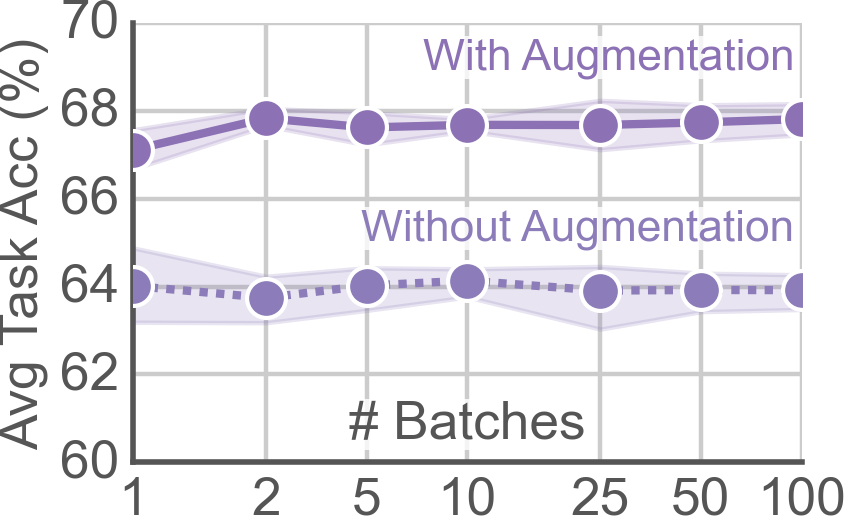
\includegraphics[width=\linewidth]{figures/imgs/cifar100_data.png}
% \end{center}
% }\end{minipage}
% }
% \subfloat[
%     \textbf{ImageNet-1k (200+200).}
%     \label{fig:data_use_imagenet}
% ]{
% \centering
% \begin{minipage}{0.48\linewidth}{
% \begin{center}
%     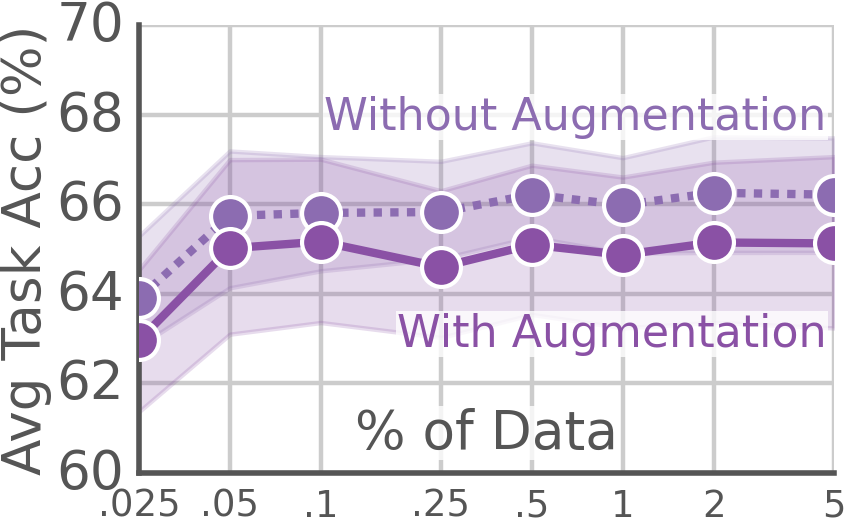
\includegraphics[width=\linewidth]{figures/imgs/imnet200_data.png}
% \end{center}
% }\end{minipage}
% }
%         \caption{
%         {\bf Data Usage.} How much data do we need to use to compute activations? Here we ablate the amount of data used for our CIFAR-100 (50+50) ResNet-20 ($8\times$ width) and ImageNet (200+200) Resnet-50 (\sfrac{22}{50} layers) experiments. The batch size used is 500 for CIFAR and 16 for ImageNet. In both cases, we only need a few hundred images to obtain the best results. On the other hand, data augmentation is necessary for CIFAR but hurts for ImageNet. Our default for all experiments uses data augmentation and the full set for CIFAR (100 batches) and 1\% of the data for ImageNet. 
%         }
% \label{fig:data_usage}
% }\end{minipage}
% \end{wrapfigure}


% \caption{{\bf Data Usage.} How much data do we need to use to compute activations? Here we ablate the amount of data used for our CIFAR-100 (50+50) ResNet-20 ($8\times$ width) and ImageNet (200+200) Resnet-50 (\sfrac{22}{50} layers) experiments. The batch size used is 500 for CIFAR and 16 for ImageNet. In both cases, we only need a few hundred images to obtain the best results. On the other hand, data augmentation is necessary for CIFAR but hurts for ImageNet. Our default for all experiments uses data augmentation and the full set for CIFAR (100 batches) and 1\% of the data for ImageNet. }
% \label{fig:data_usage}
% \end{figure}


% \begin{figure}
%     \begin{minipage}[t]{0.50\linewidth}
%         \centering
%         \subfloat[
%             \textbf{CIFAR-100 (50+50).}
%             \label{fig:partial_zip_cifar100}
%         ]{
%             \centering
%             \begin{minipage}{0.40\linewidth}{
%                 \centering
%                 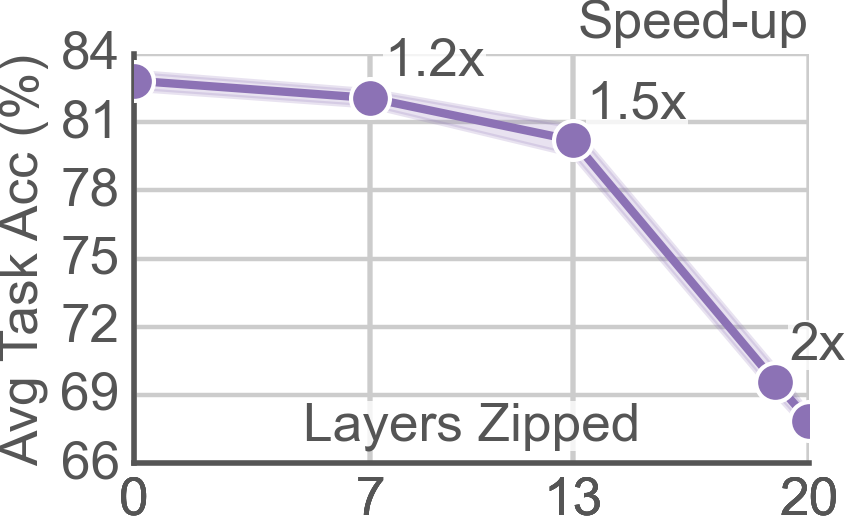
\includegraphics[width=\linewidth]{figures/imgs/partial_zip_CIFAR_50_50.png}
%             }\end{minipage}
%         }
%         \subfloat[
%             \textbf{ImageNet-1k (200+200).}
%             \label{fig:partial_zip_imagenet}
%         ]{
%             \centering
%             \begin{minipage}{0.40\linewidth}{
%                 \centering
%                 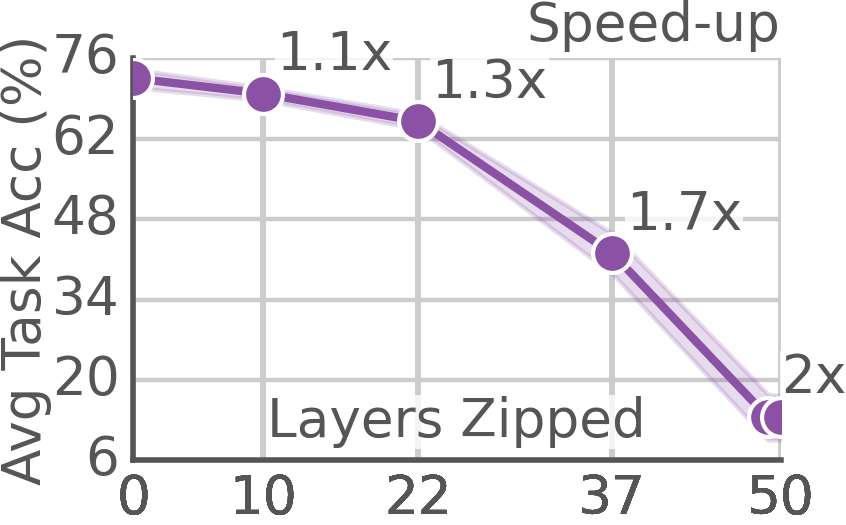
\includegraphics[width=\linewidth]{figures/imgs/partial_zip_imnet_200_200.png}
%             }\end{minipage}
%         }
%         \caption{{\bf Varying Partial Zip.} 
%             By leaving some layers unzipped (Sec.~\ref{sec:partial_zip}), we can recover a significant amount of performance while still merging most of the model.  }
%         \label{fig:varying_partial_zip}
%         % \vspace{-80pt}
%     \end{minipage}
%     \hspace{1pt}
%     % \vspace{1em} % Add vertical space between the images
%     \begin{minipage}[t]{0.48\linewidth}
%         \centering
%         \subfloat[
%             \textbf{CIFAR-100 (50+50).}
%             \label{fig:data_use_cifar100}
%         ]{
%             \centering
%             \begin{minipage}{0.48\linewidth}{
%                 \centering
%                 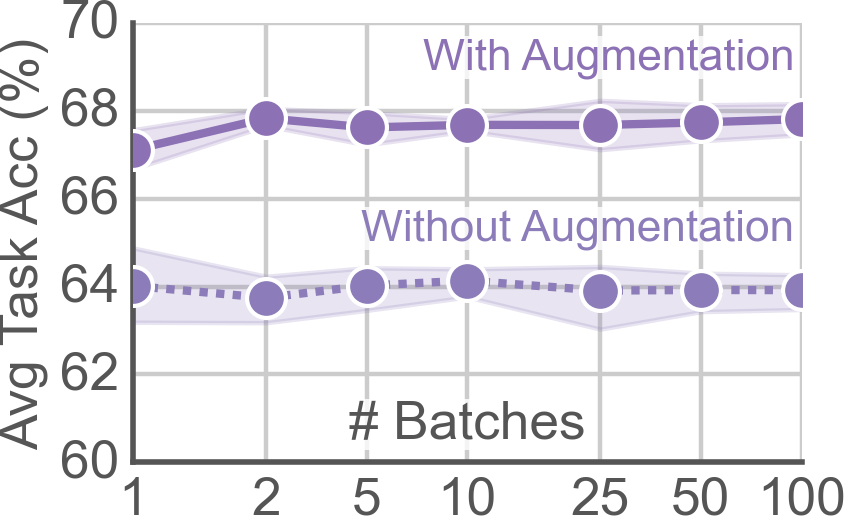
\includegraphics[width=\linewidth]{figures/imgs/cifar100_data.png}
%             }\end{minipage}
%         }
%         \subfloat[
%             \textbf{ImageNet-1k (200+200).}
%             \label{fig:data_use_imagenet}
%         ]{
%             \centering
%             \begin{minipage}{0.48\linewidth}{
%                 \centering
%                 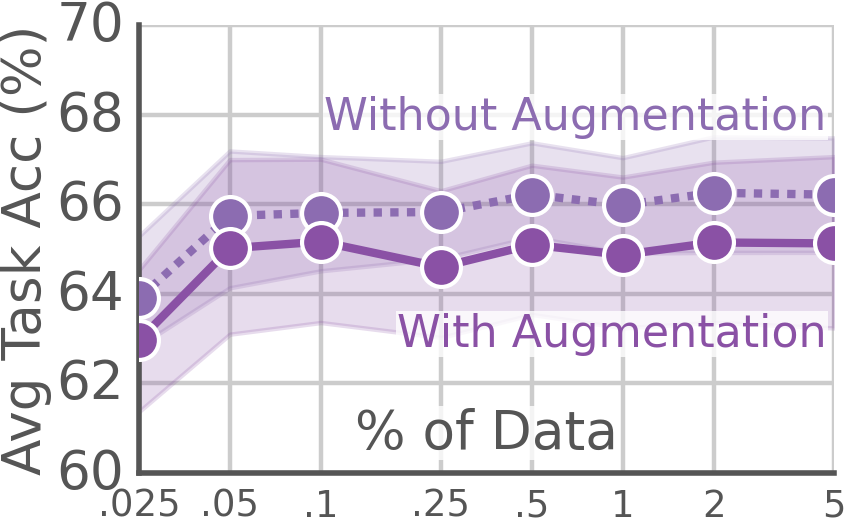
\includegraphics[width=\linewidth]{figures/imgs/imnet200_data.png}
%             }\end{minipage}
%         }
%         \caption{
%         {\bf Data Usage.} How much data do we need to use to compute activations? Here we ablate the amount of data used for our CIFAR-100 (50+50) ResNet-20 ($8\times$ width) and ImageNet (200+200) Resnet-50 (\sfrac{22}{50} layers) experiments. The batch size used is 500 for CIFAR and 16 for ImageNet. In both cases, we only need a few hundred images to obtain the best results. On the other hand, data augmentation is necessary for CIFAR but hurts for ImageNet. Our default for all experiments uses data augmentation and the full set for CIFAR (100 batches) and 1\% of the data for ImageNet. 
%         }
%         \label{fig:data_usage}
%         % \vspace{10pt}
%     \end{minipage}
%     % \caption{Overall caption for the three images}
%     \vspace{-20pt}
% \end{figure}

% \begin{wrapfigure}{r}{0.48\linewidth}
% \vspace{-10pt}
% \centering
% \resizebox{\linewidth}{!}{
%     \tablestyle{5pt}{1.1}
%     {
%     \tablestyle{5pt}{1.1}
%     \begin{tabular}{x{40}x{40}x{40}}
%         \multicolumn{3}{c}{Average Stage Correlations}\\
%         Layer \sfrac{7}{20} & Layer \sfrac{13}{20} & Layer \sfrac{19}{20}\\
%     \shline
%     {0.50\conf{0.01}} & {0.37\conf{0.00}} & {0.27\conf{0.00}} \\
%     \hline
% \end{tabular}
%     }
% }
% \captionof{table}{\textbf{CIFAR-100 (50+50) Zipping Correlations.} We show the average correlations between two ResNet-20 ($8\times$) models at each partial zipping stage. Correlations consistently decrease at each successive stage, indicating that the layers of the two models increasingly diverge. 
% }
% \label{tab:partialzip_corrs}
% % \end{table}
% \vspace{-20pt}
% \end{wrapfigure}



\section{Data Usage} \label{ap:data_usage}
In our approach, we use a sample of the training set in order to compute activations and match features together. For the main paper, we used the full training set for CIFAR, 1\% of the training set for ImageNet, and the number of images in the smallest training set for the Multi-Dataset classification experiment (so that we could use the same number of images from each dataset). In each case, we used the same data augmentations from training.

That begs the question: how much data do we actually need, and how necessary are data augmentations?
Here we ablate the amount of data used for our CIFAR-100 (50+50) ResNet-20 ($8\times$ width) and ImageNet (200+200) Resnet-50 (\sfrac{22}{50} layers) experiments. 
In Fig.~\ref{fig:data_usage}, we test how much data is actually necessary to obtain a good accuracy on CIFAR and ImageNet with or without data augmentation.

% \begin{figure}[h]
% \centering
% %
% \subfloat[
%     \textbf{CIFAR-100 (50+50).}
%     \label{fig:data_use_cifar100}
% ]{
% \centering
% \begin{minipage}{0.48\linewidth}{
% \begin{center}
%     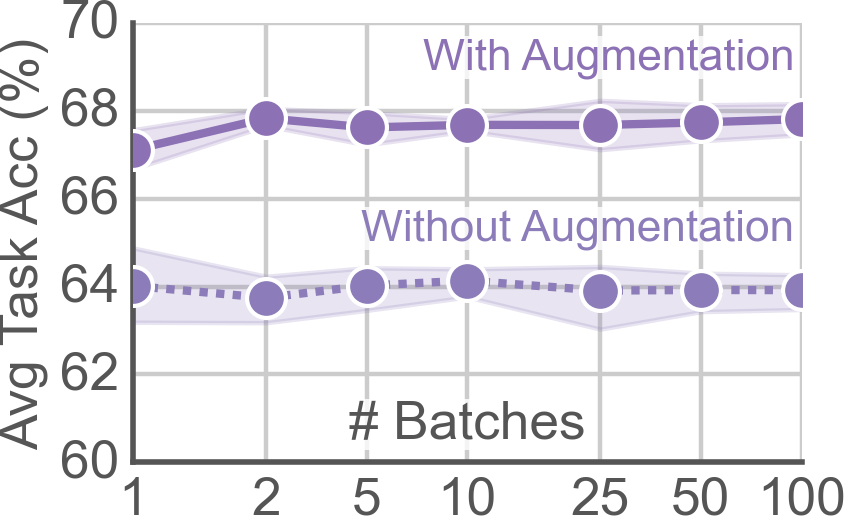
\includegraphics[width=\linewidth]{figures/imgs/cifar100_data.png}
% \end{center}
% }\end{minipage}
% }
% \subfloat[
%     \textbf{ImageNet-1k (200+200).}
%     \label{fig:data_use_imagenet}
% ]{
% \centering
% \begin{minipage}{0.48\linewidth}{
% \begin{center}
%     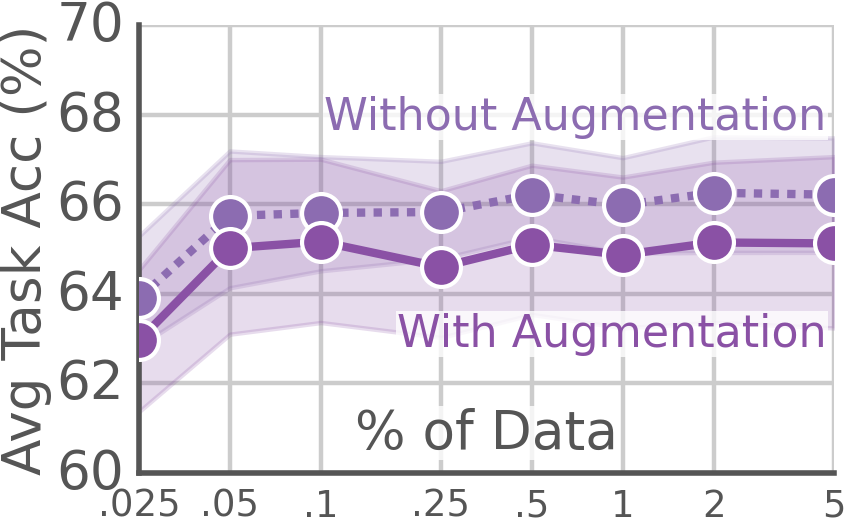
\includegraphics[width=\linewidth]{figures/imgs/imnet200_data.png}
% \end{center}
% }\end{minipage}
% }

% \caption{{\bf Data Usage.} How much data do we need to use to compute activations? Here we ablate the amount of data used for our CIFAR-100 (50+50) ResNet-20 ($8\times$ width) and ImageNet (200+200) Resnet-50 (\sfrac{22}{50} layers) experiments. The batch size used is 500 for CIFAR and 16 for ImageNet. In both cases, we only need a few hundred images to obtain the best results. On the other hand, data augmentation is necessary for CIFAR but hurts for ImageNet. Our default for all experiments uses data augmentation and the full set for CIFAR (100 batches) and 1\% of the data for ImageNet. }
% \label{fig:data_usage}
% \end{figure}



% \begin{wrapfigure}{l}{0.52\linewidth}
% % \vspace{-260pt}
% \begin{minipage}[l]{\linewidth}{
% \subfloat[
%     \textbf{CIFAR-100 (50+50).}
%     \label{fig:data_use_cifar100}
% ]{
% \centering
% \begin{minipage}{0.48\linewidth}{
% \begin{center}
%     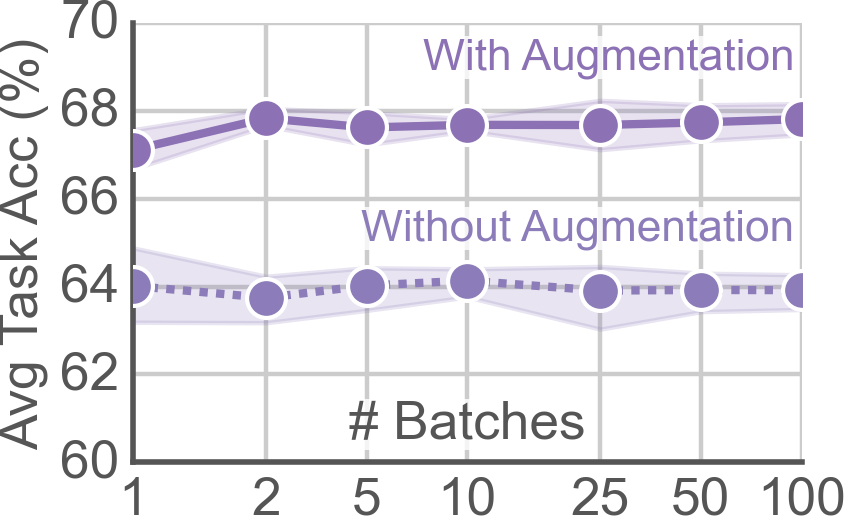
\includegraphics[width=\linewidth]{figures/imgs/cifar100_data.png}
% \end{center}
% }\end{minipage}
% }
% \subfloat[
%     \textbf{ImageNet-1k (200+200).}
%     \label{fig:data_use_imagenet}
% ]{
% \centering
% \begin{minipage}{0.48\linewidth}{
% \begin{center}
%     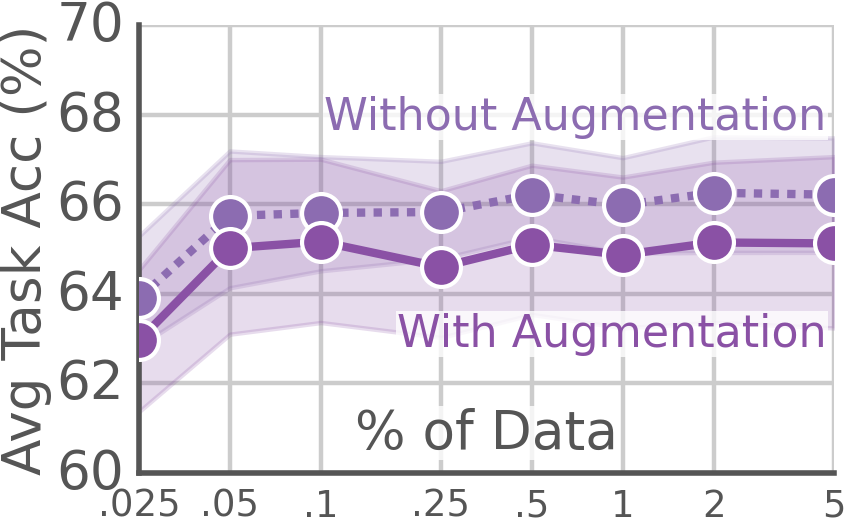
\includegraphics[width=\linewidth]{figures/imgs/imnet200_data.png}
% \end{center}
% }\end{minipage}
% }
%         \caption{
%         {\bf Data Usage.} How much data do we need to use to compute activations? Here we ablate the amount of data used for our CIFAR-100 (50+50) ResNet-20 ($8\times$ width) and ImageNet (200+200) Resnet-50 (\sfrac{22}{50} layers) experiments. The batch size used is 500 for CIFAR and 16 for ImageNet. In both cases, we only need a few hundred images to obtain the best results. On the other hand, data augmentation is necessary for CIFAR but hurts for ImageNet. Our default for all experiments uses data augmentation and the full set for CIFAR (100 batches) and 1\% of the data for ImageNet. 
%         }
% \label{fig:data_usage}
% }\end{minipage}
% \end{wrapfigure}

We ultimately find that the amount of data doesn't actually matter that much. In the main paper, we use the entire training set for CIFAR-100 with a batch size of 500 (100 batches, or 50,000 images), but it seems like as little as 2 batches (100 images) produces the same result. Similarly on ImageNet, using 0.05\% of the data (640 images) produces the same result as 5\% (64,048 images).

In fact, the main consideration is whether or not to use data augmentation. For less diverse datasets like CIFAR-100, data augmentation seems essential (giving an almost 4\% boost in average task accuracy), and well above the variance of results without augmentation. However, for ImageNet, which has much more diverse images, data augmentation actually hurts slightly on average---though the two are within variance. Note that despite this result, for consistency we use data augmentation in \textit{all} experiments.


\section{Zip Propagation Details} \label{ap:prop_rules}
In the main paper we described general rules for zip propagation---namely, propagate through layers until you reach a module with a weight matrix. Here, we describe rules more concretely for each layer type needed to define most convnets.

\paragraph{Linear.} Apply \modelc{$M_i$} and \modelc{$U_i$}. Stop propagation.

\paragraph{Conv.} Apply \modelc{$M_i$} and \modelc{$U_i$} to each kernel location (i.e., move the $k\times k$ kernel dimensions to the batch dimension). Stop propagation.

\paragraph{BatchNorm.} Apply \modelc{$M_i$} to all parameters (weight, bias, mean, variance), squaring it for the variance term. Continue propagation. As \citet{jordan2022repair} points out, we cannot compute the correct variance without knowing the covariance between the two models (which we don't have access to). Thus, we reset batch norms after merging to evaluate the variance correctly. 

\paragraph{LayerNorm.} Apply \modelc{$M_i$} to all parameters (weight, bias). Continue propagation. Since LayerNorm computes mean and standard deviation on the fly, we don't need to do anything special.

\paragraph{ReLU.} Nothing to merge. Continue propagation. Note that passing the merge matrix unchanged through the ReLU layers is an approximation, since we're using a linear merge operation on nonlinear features. Addressing this issue could be an interesting topic for future work, as even the permute and add approach of prior work has this issue (ReLU is invariant to permutation, but certainly not adding). 

\paragraph{Avg / Max Pool.} Nothing to Merge. Continue propagation.

\paragraph{Skip Connection.} Continue propagation through every input to the skip connection (using the same \modelc{$M_i$} and \modelc{$U_i$} for each).


\section{Cross Entropy on CIFAR}
% %##################################################################################################
% \begin{wrapfigure}{r}{0.48\linewidth}
% % \vspace{-10pt}
% % \begin{table}[t]
% \resizebox{\linewidth}{!}{
%     \tablestyle{5pt}{1.1}
%     {\renewcommand\conf[1]{}
%     \tablestyle{5pt}{1.1}
% \centering
% \begin{center}
% \tablestyle{5pt}{1.1}
% \begin{tabular}{y{56}x{40}|x{30}x{30}x{30}x{30}}
%         & & \multicolumn{4}{c}{Accuracies (\%)}\\
%         Method & FLOPs (G) & Joint & \modela{Task A} & \modelb{Task B} & Avg \\
%     \shline
%     \modela{Model A}                        & {10.88} & {37.9\conf{0.2}} & {74.15\conf{0.6}} & {1.7\conf{0.3}} & {36.4\conf{0.7}} \\
%     \modelb{Model B}                        & {10.88} & {36.7\conf{1.2}} & {2.2\conf{0.5}} & {75.2\conf{2.3}} & {38.7\conf{1.1}} \\
%     \hline
%     W. Avg                                  &  10.88     & {2.7\conf{0.1}}           & {5.0\conf{3.3}}           & {4.9\conf{1.2}}           & {4.9\conf{0.1}} \\
%     Git Re-Basin$\ddag$                     &  10.88     & {3.1\conf{0.8}}           & {5.8\conf{0.9}}           & {5.3\conf{0.8}}           & {5.6\conf{0.8}}  \\
%     Permute                                 &  10.88     & {20.0\conf{1.3}}          & {30.8\conf{3.3}}          & {32.8\conf{1.6}}          & {31.8\conf{1.7}} \\
%     \default{{\bf \name{}}$_\text{20/20}$}  &  10.88     & \textbf{27.9\conf{1.5}}   & \textbf{40.1\conf{2.4}}   & \textbf{39.7\conf{1.6}}   & \textbf{39.9\conf{1.9}} \\
%     \hline
%     \gc{Ensemble}                           & \gc{21.76} & \gc{60.5\conf{1.0}}       & \gc{74.2\conf{0.6}}       & \gc{75.2\conf{2.3}}       &  \gc{74.7\conf{1.4}} \\
%     \default{{\bf \name{}}$_\text{13/20}$}  & {14.52}    & {38.6\conf{2.4}}          & {51.8\conf{1.6}}          & {52.0\conf{3.5}}          & {51.9\conf{2.4}} \\
%     \default{{\bf \name{}}$_\text{7/20}$}   & {18.14}    &  \textbf{47.0\conf{2.2}}         &  \textbf{60.6\conf{1.2}}         & \textbf{60.5\conf{3.2}}          & \textbf{60.6\conf{2.1}} \\
% \end{tabular}
% \end{center}
% % \end{table}
% }
% }
% \caption{\textbf{CIFAR-100 (50+50) with Cross Entropy.} \name{}\ vs. baselines using ResNet-20 ($16\times$ width). Merging the entire model as in prior work produces bad results when using cross-entropy, hence we use CLIP in the main draft. If we use partial zipping, we can recover a lot of the lost performance. $\ddag$ refers to \cite{ainsworth2022git}
% }
% % \vspace{-20pt}
% \label{tab:cifar_ce_results}
% \end{wrapfigure}

\begin{wrapfigure}{r}{0.48\linewidth}
\vspace{-10pt}
\centering
\resizebox{\linewidth}{!}{
    \tablestyle{5pt}{1.1}
    {\renewcommand\conf[1]{}
    \tablestyle{5pt}{1.1}
    \begin{tabular}{y{56}x{40}|x{30}x{30}x{30}x{30}}
        & & \multicolumn{4}{c}{Accuracies (\%)}\\
        Method & FLOPs (G) & Joint & \modela{Task A} & \modelb{Task B} & Avg \\
    \shline
    \modela{Model A}                        & {10.88} & {37.9\conf{0.2}} & {74.15\conf{0.6}} & {1.7\conf{0.3}} & {36.4\conf{0.7}} \\
    \modelb{Model B}                        & {10.88} & {36.7\conf{1.2}} & {2.2\conf{0.5}} & {75.2\conf{2.3}} & {38.7\conf{1.1}} \\
    \hline
    W. Avg                                  &  10.88     & {2.7\conf{0.1}}           & {5.0\conf{3.3}}           & {4.9\conf{1.2}}           & {4.9\conf{0.1}} \\
    Git Re-Basin$\ddag$                     &  10.88     & {3.1\conf{0.8}}           & {5.8\conf{0.9}}           & {5.3\conf{0.8}}           & {5.6\conf{0.8}}  \\
    Permute                                 &  10.88     & {20.0\conf{1.3}}          & {30.8\conf{3.3}}          & {32.8\conf{1.6}}          & {31.8\conf{1.7}} \\
    \default{{\bf \name{}}$_\text{20/20}$}  &  10.88     & \textbf{27.9\conf{1.5}}   & \textbf{40.1\conf{2.4}}   & \textbf{39.7\conf{1.6}}   & \textbf{39.9\conf{1.9}} \\
    \hline
    \gc{Ensemble}                           & \gc{21.76} & \gc{60.5\conf{1.0}}       & \gc{74.2\conf{0.6}}       & \gc{75.2\conf{2.3}}       &  \gc{74.7\conf{1.4}} \\
    \default{{\bf \name{}}$_\text{13/20}$}  & {14.52}    & {38.6\conf{2.4}}          & {51.8\conf{1.6}}          & {52.0\conf{3.5}}          & {51.9\conf{2.4}} \\
    \default{{\bf \name{}}$_\text{7/20}$}   & {18.14}    &  \textbf{47.0\conf{2.2}}         &  \textbf{60.6\conf{1.2}}         & \textbf{60.5\conf{3.2}}          & \textbf{60.6\conf{2.1}} \\
\end{tabular}
    }
}
\captionof{table}{\textbf{CIFAR-100 (50+50) Cross Entropy.} \name{}\ vs. baselines using ResNet-20 ($16\times$ width). Merging the entire model as in prior work produces bad results when using cross-entropy, hence we use CLIP in the main draft. If we use partial zipping, we can recover a lot of the lost performance. $\ddag$ refers to \cite{ainsworth2022git}
% all pairs (2-way merging) and per-task accuracy for each head (4-way merging).
% We compare to our strong baseline as \cite{ainsworth2022git} doesn't support models with different outputs.
}
\label{tab:cifar_ce_results}
% \end{table}
\vspace{-20pt}
\end{wrapfigure}

% different run 
% \begin{center}
% \tablestyle{5pt}{1.1}
% \begin{tabular}{y{56}x{20}x{28}|x{24}x{24}x{24}}
%     & FLOPs& Joint & \multicolumn{3}{c}{Per-Task (\%)}\\
%     Method & (G) & Acc (\%) & \modela{Task A} & \modelb{Task B} & Avg\\
%     \shline
%     \modela{Model A}                        & {10.88} & {33.3\conf{0.7}} & {36.3\conf{0.4}} & {70.6\conf{1.3}} & {2.03\conf{0.7}} \\
%     \modelb{Model B}                        & {10.88} & {35.8\conf{1.1}} & {36.8\conf{1.1}} & {1.9\conf{0.5}} & {71.7\conf{2.3}} \\
%     \hline
%     W. Avg                                  &  10.88     & {6.7\conf{0.7}}           & {9.5\conf{0.7}}           & {0.1\conf{4.6}}           & {11.0\conf{5.4}} \\
%     Git Re-Basin \cite{ainsworth2022git}    &  10.88     & {1.0\conf{0.0}}           & {2.1\conf{0.1}}           & {2.0\conf{0.1}}           & {2.1\conf{0.1}}  \\
%     Permute                                 &  10.88     & {31.5\conf{3/3}}          & {46.0\conf{3.7}}          & {45.9\conf{3.2}}          & {46.0\conf{6.5}} \\
%     \default{{\bf \name{}}$_\text{20/20}$}  &  10.88     & \textbf{38.2\conf{1.5}}   & \textbf{52.5\conf{2.0}}   & \textbf{52.0\conf{2.9}}   & \textbf{52.9\conf{4.0}} \\
%     \hline
%     \gc{Ensemble}                           & \gc{21.76} & \gc{54.8\conf{1.1}}       & \gc{71.2\conf{1.2}}       & \gc{70.6\conf{1.3}}       &  \gc{71.7\conf{2.3}} \\
%     \default{{\bf \name{}}$_\text{13/20}$}  & {14.52}    & {51.2\conf{1.1}}          & {67.4\conf{1.2}}          & {66.7\conf{2.0}}          & {68.2\conf{1.9}} \\
%     \default{{\bf \name{}}$_\text{7/20}$}   & {18.14}    &  \textbf{51.6\conf{0.4}}         &  \textbf{67.5\conf{0.8}}         & \textbf{66.9\conf{2.3}}          & \textbf{68.0\conf{1.4}} \\
% \end{tabular}
% \end{center}
% % }\end{minipage}
% % }

% \caption{\textbf{CIFAR-100 (50+50) with Cross Entropy.} \name{}\ vs. baselines using ResNet-20 ($16\times$ width). Merging the entire model as in prior work produces bad results when using cross-entropy, hence we use CLIP in the main draft. If we use partial zipping, we can recover a lot of the lost performance.
% }
% \label{tab:cifar_results}
% \end{table}




% \begin{table}[t]
% \centering
% \tablestyle{5pt}{1.1}
% \begin{tabular}{y{56}x{20}x{28}|x{24}x{24}x{24}}
%     & FLOPs& Joint & \multicolumn{3}{c}{Per-Task (\%)}\\
%     Method & (G) & Acc (\%) & \modela{Task A} & \modelb{Task B} & Avg\\
%     \shline
%     \modela{Model A} & {2.72} & {33.0\conf{1.2}} & {68.1\conf{0.5}} & {1.7\conf{0.3}} & {34.9\conf{0.2}} \\
%     \modelb{Model B} & {2.72} & {35.6\conf{0.5}} & {1.7\conf{0.4}} & {71.6\conf{0.8}} & {36.7\conf{0.5}} \\
%     \hline
%     W. Avg \tiny{(Eq.~\ref{eq:wavg})} &2.72& {1.3\conf{.1}} & {2.8\conf{0.5}} & {2.6\conf{0.3}} & {2.7\conf{0.2}} \\
%     Git Re-Basin \cite{ainsworth2022git}  &2.72 & {1.7\conf{0.4}} & {2.9\conf{0.5}} & {3.5\conf{0.5}} & {3.2\conf{0.5}}  \\
%     Permute \tiny{(Eq.~\ref{eq:rebasin})} &2.72 & \textbf{9.2\conf{0.9}} & \textbf{14.9\conf{0.6}} & \textbf{17.2\conf{1.9}} & \textbf{16.1\conf{1.2}} \\
%     \default{{\bf \name{}}$_\text{20/20}$} &2.72 & \textbf{8.4\conf{0.9}} & \textbf{14.5\conf{1.7}} & \textbf{15\conf{1.2}} & \textbf{14.8\conf{1.4}} \\
%     \hline
%     \gc{Ensemble} & \gc{5.45} & \gc{55.7\conf{1.5}} & \gc{68.1\conf{2.3}} & \gc{71.6\conf{0.8}} & \gc{69.8\conf{1.5}} \\
%     \default{{\bf \name{}}$_\text{13/20}$} & 3.63 & {25.0\conf{2.0}} & {24.5\conf{0.8}} & {26.8\conf{2.2}} & {25.6\conf{1.3}} \\
% \end{tabular}

% \caption{\textbf{CIFAR50+50 ResNet20x8 Results.}
% }
% \label{tab:r20x8_c50logits}
% \end{table}
% %##################################################################################################
In the main paper, we train our CIFAR models with a CLIP \cite{radford2021learning} loss (using CLIP embeddings of class names as targets). This ensures that the output spaces of the two models are aligned, which is necessary to get good accuracy for prior work that merge the entire model together. 

\paragraph{ResNet.} In Tab.~\ref{tab:cifar_ce_results}, we show results for CIFAR-100 (50+50) where we train with the normal one-hot targets (i.e., like we did for ImageNet), instead. Immediately, we see that accuracies of the merged models are much lower across the board, with no method able to outperform just using one of the original models when merging the entire network. In fact, Git Re-Basin \cite{ainsworth2022git} does almost no better than weight averaging, which gets close to random accuracy. While \name{}\ without partial zipping also performs worse than the original models, it still greatly outperforms all prior work. And with partial zipping, \name{}\ is able to exceed the accuracy of the original models.

Thus, in the case of using cross-entropy loss, partial zipping is extremely important. Merging the entire model as in prior work fails, since the later layers of the model are incompatible with each other due to each model having a different output space. Partial zipping, on the other hand, can mitigate that issue.


% %##################################################################################################
% \begin{table}[t]
% \centering
% \begin{center}
% \tablestyle{5pt}{1.1}
% \begin{tabular}{y{56}x{20}x{28}|x{24}x{24}x{24}}
%     & FLOPs& Joint & \multicolumn{3}{c}{Per-Task (\%)}\\
%     Method & (G) & Acc (\%) & \modela{Task A} & \modelb{Task B} & Avg\\
%     \shline
%     \modela{Model A}                        & {0.15} & {44.6\conf{1.0}} & {89.2\conf{2.0}} & {21.0\conf{1.5}} & {55.1\conf{1.5}} \\
%     \modelb{Model B}                        & {0.15} & {44.0\conf{1.4}} & {23.1\conf{4.5}} & {88.1\conf{2.8}} & {55.6\conf{3.4}} \\
%     \hline
%     W. Avg                                  &  0.15     & {10.2\conf{0.2}}           & {20.8\conf{1.2}}           & {20.9\conf{0.7}}           & {20.9\conf{0.7}} \\
%     Permute                                 &  0.15     & {25.4\conf{1.1}}          & {47.2\conf{1.3}}          & {48.5\conf{12.3}}          & {47.8\conf{5.8}} \\
%     \default{{\bf \name{}}$_\text{22/22}$}  &  0.15     & \textbf{33.2\conf{9.3}}   & \textbf{53.8\conf{14.7}}   & \textbf{59.9\conf{9.6}}   & \textbf{56.5\conf{6.5}} \\
%     \hline
%     \gc{Ensemble}                           & \gc{0.30} & \gc{66.6\conf{2.5}}       & \gc{89.2\conf{2.0}}       & \gc{88.1\conf{2.8}}       &  \gc{88.6\conf{0.5}} \\
%     \default{{\bf \name{}}$_\text{14/22}$}  & {0.17}    & {35.2\conf{6.0}}          & {56.7\conf{13.7}}          & {60.2\conf{15.9}}          & {58.4\conf{5.9}} \\
%     \default{{\bf \name{}}$_\text{7/22}$}   & {0.27}    &  \textbf{44.5\conf{2.9}}  &  \textbf{66.0\conf{4.2}}    & \textbf{65.1\conf{11.2}} & \textbf{65.5\conf{4.1}} \\
% \end{tabular}
% \end{center}
% % }\end{minipage}
% % }

% \caption{\textbf{CIFAR-10 (5+5) CE with VGG.} \name{}\ vs. baselines using VGG11 ($1\times$ width) using Cross Entropy instead of CLIP loss. \name{} displays the same behavior here as it does for ResNet-20 with low width. Note that this is CIFAR-10 not CIFAR-100.
% }
% \label{tab:cifar5_vgg11w1_results}
% \end{table}


\begin{wrapfigure}{r}{0.48\linewidth}
\vspace{-10pt}
\centering
\resizebox{\linewidth}{!}{
    \tablestyle{5pt}{1.1}
    {\renewcommand\conf[1]{}
    \tablestyle{5pt}{1.1}
    \begin{tabular}{y{56}x{40}|x{30}x{30}x{30}x{30}}
        & & \multicolumn{4}{c}{Accuracies (\%)}\\
        Method & FLOPs (G) & Joint & \modela{Task A} & \modelb{Task B} & Avg \\
    \shline
    \modela{Model A}                        & {0.15} & {44.6\conf{1.0}} & {89.2\conf{2.0}} & {21.0\conf{1.5}} & {55.1\conf{1.5}} \\
    \modelb{Model B}                        & {0.15} & {44.0\conf{1.4}} & {23.1\conf{4.5}} & {88.1\conf{2.8}} & {55.6\conf{3.4}} \\
    \hline
    W. Avg                                  &  0.15     & {10.2\conf{0.2}}           & {20.8\conf{1.2}}           & {20.9\conf{0.7}}           & {20.9\conf{0.7}} \\
    Permute                                 &  0.15     & {25.4\conf{1.1}}          & {47.2\conf{1.3}}          & {48.5\conf{12.3}}          & {47.8\conf{5.8}} \\
    \default{{\bf \name{}}$_\text{22/22}$}  &  0.15     & \textbf{33.2\conf{9.3}}   & \textbf{53.8\conf{14.7}}   & \textbf{59.9\conf{9.6}}   & \textbf{56.5\conf{6.5}} \\
    \hline
    \gc{Ensemble}                           & \gc{0.30} & \gc{66.6\conf{2.5}}       & \gc{89.2\conf{2.0}}       & \gc{88.1\conf{2.8}}       &  \gc{88.6\conf{0.5}} \\
    \default{{\bf \name{}}$_\text{14/22}$}  & {0.17}    & {35.2\conf{6.0}}          & {56.7\conf{13.7}}          & {60.2\conf{15.9}}          & {58.4\conf{5.9}} \\
    \default{{\bf \name{}}$_\text{7/22}$}   & {0.27}    &  \textbf{44.5\conf{2.9}}  &  \textbf{66.0\conf{4.2}}    & \textbf{65.1\conf{11.2}} & \textbf{65.5\conf{4.1}} \\
\end{tabular}
    }
}
\captionof{table}{\textbf{CIFAR-10 (5+5) CE with VGG.} \name{}\ vs. baselines using VGG11 ($1\times$ width) using Cross Entropy instead of CLIP loss. \name{} displays the same behavior here as it does for ResNet-20 with low width. 
% Note that this is CIFAR-10 not CIFAR-100.
% all pairs (2-way merging) and per-task accuracy for each head (4-way merging).
% We compare to our strong baseline as \cite{ainsworth2022git} doesn't support models with different outputs.
}
\label{tab:cifar5_vgg11w1_results}
% \end{table}
\vspace{-10pt}
\end{wrapfigure}

\paragraph{VGG.}\label{ap:vgg}
In the main paper, we use ResNets for each experiment, since they are easy to train and produce strong results. However, in principle \name{}\ can work on any architecture. For completeness, in Tab.~\ref{tab:cifar5_vgg11w1_results}, we show results on the CIFAR-10 (5+5) setting with VGG11 ($1\times$ width). Note that this is a much smaller and weaker model than the ResNet-20s we use in the main paper, so its results on CIFAR-10 aren't as strong. Furthermore, we conducted this experiment with a cross entropy loss, so merging the entire model performs worse than the original models.

Despite this, we observe a very similar trend to the ResNet-20 models in that \name{}\ outperforms all baselines and that partial zipping is important for reaching the accuracy of the original models (in this case, matching not exceeding). In fact, these results continue a more general trend in that \name{}\ greatly benefits from larger model scales, making effective use of the extra capacity. In this case, the scale of the model is quite small, so there is not as much room in the weights to store the potentially disjoint features of both models.


% \begin{table}[t]
% \centering
% \tablestyle{5pt}{1.1}
% \begin{tabular}{y{56}x{20}x{28}|x{24}x{24}x{24}}
%     & FLOPs& Joint & \multicolumn{3}{c}{Per-Task (\%)}\\
%     Method & (G) & Acc (\%) & \modela{Task A} & \modelb{Task B} & Avg\\
%     \shline
%     \multicolumn{6}{c}{$1\times$ Width} \\
%     \hline
%     \gc{Ensemble} & \gc{8.22} & \gc{63.3\conf{4.9}} & \gc{74.3\conf{4.0}} & \gc{70.5\conf{3.2}} & \gc{72.4\conf{2.5}} \\
%     \default{{\bf \name{}}$_\text{50/50}$} & 4.11 & {8.6\conf{4.7}} & {12.4\conf{5.9}} & {14.7\conf{7.8}} & {13.5\conf{6.6}} \\
%     \default{{\bf \name{}}$_\text{37/50}$} & 4.92 & {33.1\conf{5.9}} & {41.8\conf{5.3}} & {42.3\conf{8.2}} & {42.0\conf{6.2}} \\
%     \default{{\bf \name{}}$_\text{22/50}$} & 6.39 & {55.8\conf{4.1}} & {65.9\conf{2.5}} & {64.1\conf{3.0}} & {65.0\conf{2.3}} \\
%     \default{{\bf \name{}}$_\text{10/50}$} & 7.43 & {60.9\conf{4.1}} & {70.7\conf{3.0}} & {69.0\conf{2.9}} & {69.9\conf{1.9}} \\
%     \hline
%     \multicolumn{6}{c}{$1.5\times$ Width} \\
%     \hline
%     \gc{Ensemble} & \gc{32.6} & \gc{67.8\conf{3.5}} & \gc{76.7\conf{4.1}} & \gc{72.6\conf{2.8}} & \gc{74.7\conf{2.5}} \\
%     \default{{\bf \name{}}$_\text{50/50}$} & 16.3 & {9.7\conf{6.9}} & {13.2\conf{9.5}} & {16.0\conf{10.0}} & {14.6\conf{9.3}} \\
%     \default{{\bf \name{}}$_\text{37/50}$} & 19.5 & {49.0\conf{2.5}} & {56.2\conf{4.2}} & {56.7\conf{2.1}} & {56.4\conf{2.8}} \\
%     \default{{\bf \name{}}$_\text{22/50}$} & 25.5 & {64.1\conf{2.7}} & {71.6\conf{2.3}} & {70.4\conf{2.3}} & {71.0\conf{1.8}} \\
%     \default{{\bf \name{}}$_\text{10/50}$} & 29.7 & {66.8\conf{3.2}} & {74.9\conf{3.5}} & {72.1\conf{2.3}} & {73.5\conf{2.1}} \\
% \end{tabular}

% \caption{\textbf{ImageNet-1k (200+200) Width Comparison.} We show how \name{}\ is able to make use of the extra model width when merging models together. For instance, merging 37 layers goes from 33\% joint accuracy with $1\times$ width to 49\% with $1.5\times$, while the ensemble only improves by 4\%. Because these models use cross-entropy, merging the entire network still results in poor performance.
% }
% \label{tab:imagenet200x5width}
% \end{table}

\begin{wrapfigure}{r}{0.48\linewidth}
\vspace{-10pt}
\centering
\resizebox{\linewidth}{!}{
    \tablestyle{5pt}{1.1}
    {\renewcommand\conf[1]{}
    \tablestyle{5pt}{1.1}
    \begin{tabular}{y{56}x{40}|x{30}x{30}x{30}x{30}}
        & & \multicolumn{4}{c}{Accuracies (\%)}\\
        Method & FLOPs (G) & Joint & \modela{Task A} & \modelb{Task B} & Avg \\
    \shline
    \multicolumn{6}{c}{$1\times$ Width} \\
    \hline
    \gc{Ensemble} & \gc{8.22} & \gc{63.3\conf{4.9}} & \gc{74.3\conf{4.0}} & \gc{70.5\conf{3.2}} & \gc{72.4\conf{2.5}} \\
    \default{{\bf \name{}}$_\text{50/50}$} & 4.11 & {8.6\conf{4.7}} & {12.4\conf{5.9}} & {14.7\conf{7.8}} & {13.5\conf{6.6}} \\
    \default{{\bf \name{}}$_\text{37/50}$} & 4.92 & {33.1\conf{5.9}} & {41.8\conf{5.3}} & {42.3\conf{8.2}} & {42.0\conf{6.2}} \\
    \default{{\bf \name{}}$_\text{22/50}$} & 6.39 & {55.8\conf{4.1}} & {65.9\conf{2.5}} & {64.1\conf{3.0}} & {65.0\conf{2.3}} \\
    \default{{\bf \name{}}$_\text{10/50}$} & 7.43 & {60.9\conf{4.1}} & {70.7\conf{3.0}} & {69.0\conf{2.9}} & {69.9\conf{1.9}} \\
    \hline
    \multicolumn{6}{c}{$1.5\times$ Width} \\
    \hline
    \gc{Ensemble} & \gc{32.6} & \gc{67.8\conf{3.5}} & \gc{76.7\conf{4.1}} & \gc{72.6\conf{2.8}} & \gc{74.7\conf{2.5}} \\
    \default{{\bf \name{}}$_\text{50/50}$} & 16.3 & {9.7\conf{6.9}} & {13.2\conf{9.5}} & {16.0\conf{10.0}} & {14.6\conf{9.3}} \\
    \default{{\bf \name{}}$_\text{37/50}$} & 19.5 & {49.0\conf{2.5}} & {56.2\conf{4.2}} & {56.7\conf{2.1}} & {56.4\conf{2.8}} \\
    \default{{\bf \name{}}$_\text{22/50}$} & 25.5 & {64.1\conf{2.7}} & {71.6\conf{2.3}} & {70.4\conf{2.3}} & {71.0\conf{1.8}} \\
    \default{{\bf \name{}}$_\text{10/50}$} & 29.7 & {66.8\conf{3.2}} & {74.9\conf{3.5}} & {72.1\conf{2.3}} & {73.5\conf{2.1}} \\
\end{tabular}
    }
}
\captionof{table}{\textbf{ImageNet-1k (200+200) Width Comparison.} We show how \name{}\ is able to make use of the extra model width when merging models together. For instance, merging 37 layers goes from 33\% joint accuracy with $1\times$ width to 49\% with $1.5\times$, while the ensemble only improves by 4\%. These models use cross-entropy, so merging the entire network results in poor performance.
% all pairs (2-way merging) and per-task accuracy for each head (4-way merging).
% We compare to our strong baseline as \cite{ainsworth2022git} doesn't support models with different outputs.
}
\label{tab:imagenet200x5width}
% \end{table}
\vspace{-20pt}
\end{wrapfigure}

\section{ImageNet with 1.5x Width}
In the main paper, we show that \name{}\ scales very well with increased width of the model for the CIFAR-100 (50+50) setting. While CIFAR-100 is a challenging dataset on its own, the natural question is if that same trend occurs the much harder ImageNet-1k (200+200) setting.

In Tab.~\ref{tab:imagenet200x5width}, we test this by comparing \name{}\ on the original $1\times$ width ResNet-50 in the main paper with a $1.5\times$ width one.
In all cases, except for the fully zipped model (likely because of the Cross-Entropy loss), \name{}\ enjoys a large jump in performance from the extra width. For 37 layers, 33.1\% joint accuracy becomes 49.0\%. For 22 layers, 55.8\% becomes 64.1\%. And for 10 layers, 60.9\% becomes 66.8\%, now only 1\% away from the ensemble. Thus, even in this much more challenging setting, \name{}\ is able to make full use of the extra model capacity.

\section{Merging models with different output modalities} \label{appendix:semantic_segmentation}
\begin{wrapfigure}{r}{0.48\linewidth}
\vspace{-10pt}
\centering
\resizebox{\linewidth}{!}{
    \tablestyle{5pt}{1.1}
    {\renewcommand\conf[1]{}
    \tablestyle{5pt}{1.1}
    \begin{tabular}{y{40}|x{50}x{50}} 
                                                &      {Accuracy (\%)}      &         {mIoU (\%)}       \\
        Method                                  & \modela{ImageNet-1k}      & \modelb{Pascal VOC}       \\ 
    \shline
    W. Avg                                      & {0.8}         & {3.3}         \\
    \default{{\bf \name{}}$_\text{49/50}$}      & \textbf{23.1}            & \textbf{6.0}  \\
    \hline
    \gc{Ensemble}                               & \gc{77.8}                & \gc{76.8}                \\
    \default{{\bf \name{}}$_\text{37/50}$}      & {47.7}                   & {35.0}                   \\
    \default{{\bf \name{}}$_\text{22/50}$}      & {60.9}                   & {64.4}                   \\
    \default{{\bf \name{}}$_\text{10/50}$}      &    \textbf{64.9}         & \textbf{71.7}            \\
\end{tabular}
    }
}
\captionof{table}{\textbf{PASCAL VOC and ImageNet-1k} merging models with different output modalities using a DeepLabV3 ResNet-50 backbone and ImageNet-1k Resnet-50 model.  
}
\label{tab:voc_imagenet_results}
% \end{table}
\vspace{-10pt}
\end{wrapfigure}
In this experiment we use \name{}\ to merge two models with different initializations trained on different tasks with \textit{different} output modalities: semantic segmentation and image classification. 
Specifically, we merge the ResNet-50 backbone of a DeepLabV3 \citep{chen2017deeplabv3} model finetuned on the Pascal VOC \citep{Everingham10pascalvoc} dataset, with a ResNet-50 model trained on ImageNet-1k.
While the DeepLabV3 backbone was itself pre-trained on ImageNet-1k, it was further finetuned on Pascal VOC and does not share the initialization of our classification model. Table~\ref{tab:voc_imagenet_results} shows the results of combining the two ResNet-50 models with \name{}\ at various partial merging locations. 
% We conduct a hyperparameter search over a held-out validation set sampled from each task's validation data to find the optimal $\alpha\text{, and }\beta$ for \name{}\ at each merge location. 
We evaluate the performance of each merged by reporting its ImageNet-1k accuracy, and its Pascal VOC mIoU as is standard. 
Overall, we observe that \name{}\ is capable of merging nearly half the number of ResNet-50 layers between both models while still maintaining good performance on \textit{both tasks}, all \textit{without any training}.



% Useful Commands
\newcommand{\vv}{{\mathbf{v}}}
\newcommand{\vvP}{{\mathbf{v'}}}
\newcommand{\vvPP}{{\mathbf{v''}}}
\newcommand{\vW}{{\mathbf{W}}}
\newcommand{\vWP}{{\mathbf{W'}}}
\newcommand{\vWPP}{{\mathbf{W''}}}
\newcommand{\thetar}{\bm{\theta}_r}
\newcommand{\thetah}{\bm{\theta}_h}
% Reduced Commands
\newcommand{\vvR}{{H_{m\rightarrow r}^v(\mathbf{v})}}
\DeclarePairedDelimiter{\norm}{\lVert}{\rVert} % define a "\norm" macro

\section{A Tighter Bound for Linear Mode Connectivity}\label{ap:Theorem}
In this section we demonstrate that merging models by supporting feature merges both \textit{across} and \textit{within} each, yields a tighter bound than Theorem 3.1 in \citep{entezari2021role} in its limited setting.
We first introduce necessary background from prior work, including Theorem 3.1 and a particular formalization for within-model merging borrowed from~\citep{simsek2021geometry}.
Second, we introduce Theorem 1, which produces a tighter bound on Theorem 3.1 when merging within models is allowed, and prove its validity (Section~\ref{ap:TheoremDef} \&~\ref{ap:Theorem_proof}). 
Third, we provably extend Theorem 1 to a less restrictive setting, retaining its bounds (Section~\ref{ap:theorem1_extended}).

\subsection{Background}\label{ap:Theorem_background}
We first introduce Theorem 3.1 from \citep{entezari2021role}. Second, we formalize a restricted version of within-model merging necessary for our proof using the definitions from~\cite{simsek2021geometry}. 

\subsubsection{Thoerem 3.1}\label{ap:theorem3.1}
\paragraph{The Theorem. } Let $f_{\{\vv,\vW\}}(x)=\vv^T\sigma(\vW x)$, $f_{\{\vvP,\vWP\}}(x)=\vv'^T\sigma(\vW' x)$ be two fully-connected networks with $h$ hidden units where $\sigma(\cdot)$ is ReLU activation, $\vv\in\mathbb{R}^h$ and $\vW\in\mathbb{R}^{h\times d}$ are the parameters and $x\in\mathbb{R}^d$ is the input. If each element of $\vW$ and $\vWP$ is sampled uniformly from $[-1/\sqrt{d},1/\sqrt{d}]$ and each element of $\vv$ and $\vvP$ is sampled uniformly from $[-1/\sqrt{h},1/\sqrt{h}]$, then for any $x\in\mathbb{R}^d$ such that $\norm{x}_2=\sqrt{d}$, with probability $1-\delta$ over $\vW,\vWP, \vv, \vvP$, there exist a permutation such that

\begin{equation}
    |f_{\{\alpha\vv + (1-\alpha)\vvPP, \alpha\vW+(1-\alpha)\vWPP\}}(x) - \alpha f_{\{\vv,\vW\}}(x) - (1-\alpha)f_{\{\vvP,\vWP\}}(x)| = \Tilde{O}(h^{-\frac{1}{2d+4}})\label{eq:perm_LMC}
\end{equation}

where $\vvPP,\vWPP$ are permuted version of $\vvP,\vWP$, $\alpha\in[0,1]$ is an arbitrary interpolation constant, and the left-hand-side of the equality is the amount an interpolated model differs in output compared to the interpolation of the original models. \citep{entezari2021role} show that minimizing this quantity is analogous to minimizing the barrier (as defined by~\citet{entezari2021role}) in this setting. 
This is important because it states that achieving a zero output difference is equivalent to achieving zero-barrier, which implies that two models are linearly mode connected (LMC). 

\paragraph{Implications} Theorem 3.1 states that given any two two-layer models with different random initializations, there exists a permutation for one model such that applying the permutation makes it linearly mode connected to the second with high probability, given that the networks are \textit{wide enough} (i.e. $h$ is large enough). In other words, it states that any two randomly initialized two-layer networks are LMC modulo permutation with high likelihood. \citet{entezari2021role} use this result to conjecture that most well-trained neural networks with the same architecture and trained on the same task are also LMC modulo permutation with high likelihood. 

Notably however, permutations only allow for merging \textit{across} models. We will show how adding the ability to merge \textit{within} models leads to a tighter bound than Theorem 3.1 with the same likelihood.%, or analogously the same bound but with higher likelihood. 


% \paragraph{Preserving Function Invariance Beyond Permutations.} 
\subsubsection{A Restricted Formalization of Merging Within Models}\label{ap:reducible_def}
\paragraph{The Formalization. }
Let $\bm{\theta}_h=\{\vv,\vW\}$ represent a parameter-set such that $f_{\{\vv,\vW\}}=f_{\bm{\theta}_h}$, and likewise let $\bm{\theta'}_h=\{\vvP,\vWP\}, \text{ s.t. }, f_{\{\vvP,\vWP\}}=f_{\bm{\theta'}_h}$. 
Given $\thetah$, let $\Theta_h$ denote the set of all parameter-sets with functional equivalence to $\thetah$.
This means that $\forall \theta\in\Theta_h\text{, and }\forall x\in\{x\in\mathbb{R}^d|\  \norm{x}_2=\sqrt{d}\}, f_{\bm{\theta}}(x)=f_{\bm{\thetah}}(x)$.
Similarly, let $\Theta_h'$ be the set of all parameter-sets with functional equivalence to $\thetah'$.
Following $\bm{\theta_h}$, let $\bm{\theta}_r$ be an arbitrary parameter-set for $f$ which has $r$ hidden units instead. Assume $\bm{\theta}_h$ can be reduced to some $\bm{\theta}_r, r\leq h$ in a function-invariant manner using the definition of zero-type neurons from \citep{simsek2021geometry}. This means that there are $h-r$ total combinations of (1) rows in $\vW$ that are copies of one another whose corresponding $\vv$ elements \textit{sum to $0$}, and (2) some zero-elements in $\vv$. Thus, following \citet{simsek2021geometry} there exists a function-and-loss-preserving affine transformation that reduces $\bm{\theta}_h$ to $\bm{\theta}_r$. 
% We restrict our attention to cases where this function is linear and 
We denote this function as $M_{h\rightarrow r}\in\mathbb{R}^{r\times h}$, with $M_{h\rightarrow r}(\bm{\theta}_h)=\bm{\theta}_r$. Note that when $r=h$, $M_{h\rightarrow r}$ can simply be the identity transformation.

By definition, $\thetah$ lies in the expansion manifold of $\thetar$ \citep{simsek2021geometry}. 
This means there is a similarly defined affine transformation $U_{r\rightarrow h}\in\mathbb{R}^{h\times r}$ that can expand $\thetar$ back to arbitrary $\bm{\Tilde{\theta}_h}\in\Theta_h$ lying on the expansion manifold. 
One simple way is to extend $\thetar$ to $\bm{\Tilde{\theta}_h}$ by filling the remaining $h-r$ $\vv$ elements with $0$ and the $h-r$ $\vW$ rows with arbitrary values. 
% Under the definition, these $h-r$ neurons whose incoming weight vector copies from $\vW$ and outgoing $\vv$ elements sum to zero would be considered zero-type neurons.
Because the associated $\vv$ elements for each $\vW$ row are zero, the values of each row don't impact the function output.
% Under the definition, these $h-r$ elements would be considered zero-type neurons.
Note that because $h\geq r$, $U_{r\rightarrow h}$ can assign $\thetar$ into arbitrary new indices in $\thetah$. 
Thus, $U_{r\rightarrow h}$ act as both a \textit{permutation and expansion} transformation. 
Let $T=U\circ M=U_{r\rightarrow h}(M_{h\rightarrow r}(\thetah))$ be the coupling of the reduction and expansion affine-transformations that produce new networks of width $h$ from $\thetar$. 
By definition, any $T$ is a permutation when $M$ is the identity and $U$ is the permutation matrix. 
For the remainder of this section, we assume that $T$ further contains a permutation (i.e. $T=P\circ U\circ M$ for some permutation matrix $P\in\mathbb{R}^{h\times h}$).

We will leverage the concept of zero-type neurons presented in \citep{simsek2021geometry} to obtain a tighter bound on Theorem 3.1. 

\paragraph{A Note on Novelty.} While we borrow ideas from \citet{simsek2021geometry}, our Theorem is a differs in theoretical application. 
First, \citet{simsek2021geometry} restrict their attention to overall connectivity across points within expansion manifolds. 
% They do not explore the existence of direct-linear connectivity between two arbitrary points as in Theorem 3.1. 
This is important because our Theorem and proof do not require models to lie on the \textit{same} expansion manifold to be linearly mode connected. 
% They can instead be \textit{disconnected} over each-other's manifold. 
% Second, we seek direct-linear connectivity instead of polygonal chains. 
Second, our models need not be reducible to the same $r$. 
That is, we allow for arbitrary reducibility between any two network parameter-sets. 
% Third, our setting involves a different set of models than those studied in \citet{simsek2021geometry}. 
Our theorem also differs from Theorem 3.1 in \citep{entezari2021role} in that we extend function-invariant transformations beyond the permutation matrix, and show that tighter bounds are achievable in the process. Furthermore, we show that uniformity assumptions may be relaxed while retaining the same bounds (Section \ref{ap:theorem1_extended}).

% Let $\Omega_{r\rightarrow h}(\thetar)$ denote the expansion manifold (defined in \citep{simsek2021geometry}) of $\thetar$. For simplicity, we restrict each point in the expansion manifold to be a linear transformation of $\thetar$. We define this transformation by $U_{r\rightarrow h}\in\mathbb{R}^{h\times r}$, which expands $\thetar$ from $r$ back to width $h$. One way this can be done is 

% If $M_{h\rightarrow r}(\thetah)=\thetar$ then $\thetah$ lies in the expansion manifold of $\thetar$ as defined in \citep{simsek2021geometry}. This means that

% Under certain activations such as ReLU, we can generalize Definition 3.1 with another reducible property. More specifically, any rows in $\vW$ whose outputs are a linear combination of each other after activation can also be reduced. I.e., if there exists a set $\mathbb{S}$ of rows in $\vW$ such that $\forall x\in\mathbb{R}^d\ \exists j\notin\mathbb{S}, \sigma(\vW_j x) = \sum_{i\in \mathbb{S}} \vv_i\sigma(\vW_i x)$ where $\vv_i\in\mathbb{R}_+$ are scalar weights, then $\bm{\theta}_h$ is also reducible. 

% A second observation is that for any $M_{h\rightarrow r}\in\mathbb{R}^{r\times h}$, we can define a complementary linear transformation $U_{r\rightarrow h}\in\mathbb{R}^{h\times r}$ that expands $\bm{\theta}_r$ back to some $\bm{\theta}_h$ while preserving function and loss. One intuitive way this can be done is by copying $h-r$ arbitrary elements with appropriate normalization in $\bm{\theta}_r$ to fill $\thetah$. An even simpler way is to extend $\thetar$ to $\thetah$ by filling the remaining $h-r$ width parameters with $0$. We can do this by assigning $h-r$ elements of $\vv$ to be $0$, and then fill their corresponding $h-r$ rows of $\vW$ with any arbitrary values. Note that because $h\geq r$, $U_{r\rightarrow h}$ can assign $\thetar$ into arbitrary new indices in $\thetah$. Thus, $U_{r\rightarrow h}$ act as both a \textit{permutation and expansion} transformation. 
% Let $T=U\circ M=U_{r\rightarrow h}(M_{h\rightarrow r}(\thetah))$ be the linear coupling of the reduction and extension linear-transformations that produce new networks of width $h$ from $\thetah$. By definition, any $T$ is a permutation when $M$ is the identity and $U$ is the permutation matrix. For the remainder of this section, we assume that $T$ further contains a permutation (i.e. $T=P\circ U\circ M$ for some permutation matrix $P\in\mathbb{R}^{h\times h}$).

\subsection{A theoretical Result}\label{ap:TheoremDef}
We now introduce Theorem 1, an extension of Theoerem 3.1 that yields a strictly tighter bound when the transformations $T$ from Section~\ref{ap:reducible_def} are included and $r < h$, and exactly as tight when $r=h$. We leave the proof to the next section. 

\paragraph{Theorem 1.} 
Let $f_{\{\vv,\vW\}}(x)=\vv^T\sigma(\vW x)$, $f_{\{\vvP,\vWP\}}(x)=\vv'^T\sigma(\vW' x)$ be two fully-connected networks with $h$ hidden units where $\sigma(\cdot)$ is ReLU activation, $\vv\in\mathbb{R}^h$ and $\vW\in\mathbb{R}^{h\times d}$ are the parameters and $x\in\mathbb{R}^d$ is the input. If each element of $\vW$ and $\vWP$ is sampled uniformly from $[-1/\sqrt{d},1/\sqrt{d}]$ and each element of $\vv$ and $\vvP$ is sampled uniformly from $[-1/\sqrt{h},1/\sqrt{h}]$, then for any $x\in\mathbb{R}^d$ such that $\norm{x}_2=\sqrt{d}$, with probability $1-\delta$ over $\vW,\vWP, \vv, \vvP$, there exist transformations $T,T'$ such that
\begin{align}
    &|f_{\{\alpha\Tilde{\vv} + (1-\alpha)\Tilde{\vv}', \alpha\Tilde{\vW}+(1-\alpha)\Tilde{\vW}'\}}(x) - \alpha f_{\{\vv,\vW\}}(x) - (1-\alpha)f_{\{\vv',\vW'\}}(x)| \nonumber \\
    &\leq\begin{cases}
            \Tilde{O}\left(\left(\frac{h^2}{(r+r')-h}\right)^{-\frac{1}{2d+4}}\right) & \text{, }(r+r')-h > 0 \\
            0 &\text{, otherwise}
        \end{cases}\label{eq:T_LMC}
\end{align}
where $\Tilde{\vv},\Tilde{\vW}$ are transformed versions of $\vv,\vW$ from $T$ and $\Tilde{\vv}',\Tilde{\vW}'$ are transformed versions of $\vvP,\vWP$ from $T'$ respectively. $0 < r, r' \leq h$ are the hidden unit amounts each network can be reduced to via its respective $M,M'$ transformation before being expanded back to width $h$ via $P\circ U,P'\circ U'$, where $P,P'$ are permutation matrices.

\paragraph{Implications.} Theorem 1 states that when redundancy exists and can be leveraged in a network, one can find a transformation that yields strictly lower barrier than with permutation with any $h$. Moreover, it approaches zero-barrier faster with increase in $h$ compared to permutations. Although it only explicitly holds for random initializations---like Theorem 3.1, this theoretical intuition is supported by our experimental observations. For instance it explains why algorithms like \name{} appear to converge to the ensemble exponentially faster than permutation methods in Figure \ref{fig:variations}\hyperref[fig:variations]{b}). The ensemble achieves zero-barrier, and \name{} is faster to approach it than permutation counterparts because it can reduce models with minimal deduction in performance. 
% Similar to \citet{entezari2021role}, we leave the extension to the NTK regime \citet{jacot2021ntk} to future work.



\subsection{Theorem 1 Proof}\label{ap:Theorem_proof}
We now derive our proposed Theorem 1. Theorem 1 is very similar to Theorem 3.1--- we just add the reducibility property from Section~\ref{ap:reducible_def}.
Thus, our derivation is nearly identical to their Appendix D proof.
We fully derive the novel components of Theorem 1 for clarity, while referring to Appendix D in \cite{entezari2021role} for the remaining identical derivations to avoid redundancy.

% Thus, we can make use of most of the scaffolding in Theorem 3.1's proof (Please see page 21-23 of \cite{entezari2021role}). 
Let $\thetah=\{\vv,\vW\}$ and $\thetah'=\{\vvP,\vWP\}$ respectively as defined in Section~\ref{ap:Theorem_background}. Suppose each can be reduced to some $\thetar,\thetar'$ respectively with $r\leq h$, via an appropriate $M_{h\rightarrow r}, M_{h\rightarrow r'}$ transformation. Further, let $U_{r\rightarrow h}, U_{r'\rightarrow h}$ be as defined in Section~\ref{ap:Theorem_background}, expanding $M_{h\rightarrow r}(\thetah), M_{h\rightarrow r'}(\thetah)$ back to width $h$ by filling in all $h-r, h-r'$ dimensions in $\vv,\vvP$ with $0$ respectively and all $h-r, h-r'$ dimensions in $\vW,\vWP$ with some specific values. 
Finally, let $T,T'$ be transformations defined in Section~\ref{ap:Theorem_background} with $T=P\circ U\circ M, T'=P'\circ U'\circ M'$ respectively. 

Let $\Tilde{\bm{\theta}_h}=T(\thetah)$, $\Tilde{\bm{\theta}_h'}=T'(\thetah')$ be the new parameter-sets obtained from $T, T'$ respectively, and let $\Tilde{\bm{\theta}_h}=\{\Tilde{\vv},\Tilde{\vW}\}$ and $\Tilde{\bm{\theta}_h'}=\{\Tilde{\vvP},\Tilde{\vWP}\}$. 
By definition, $\Tilde{\bm{\theta}_h}\in\Theta_h$, and $\Tilde{\bm{\theta}_h'}\in\Theta_h'$. 
From the definitions of $T,T'$, $\vW$ has $h-r$ zero $\Tilde{\vv}$ elements and $\vWP$ has $h-r'$ zero-$\Tilde{\vv}'$ elements.
Now, let us suppose that the corresponding $ h-r$ rows in $\Tilde{\vW}$ are set to copy rows in $\Tilde{\vWP}$, and similarly $h-r'$ rows in $\Tilde{\vWP}$ rows are set to copy rows in $\Tilde{\vW}$.
Now, interpolating between any non-zero element and a zero-element is equivalent to simply scaling the non-zero element: $z: \alpha 0 + (1-\alpha)z=(1-\alpha)z$. 
Thus, so long as $h\leq (h-r) + (h-r')$, we can achieve \textit{perfect} interpolation by placing $h-r$ elements from $\Tilde{\bm{\theta}}_h'$ into 
the zero-elements of $\Tilde{\bm{\theta}}_h$ and $h-(h-r) \leq h-r'$ elements from $\Tilde{\bm{\theta}}_h$ into the zero-elements of $\Tilde{\bm{\theta}}_h'$. 
This yields the zero-part of our piece-wise bound.
% Thus, we can place up to $h-r$ elements from $\Tilde{\bm{\theta}}_h'$ into the zero-elements of $\Tilde{\bm{\theta}}_h$ and $h-r'$ zero-elements from $\Tilde{\bm{\theta}}_h'$ into the elements of $\Tilde{\bm{\theta}}_h$, obtaining perfect interpolation for $(h-r) + (h-r')=2h-(r+r')$ elements.
% This leaves just $h-(2h-(r+r'))=h-2h+(r+r')=(r+r')-h$ within each model that must be matched.
% Now we have two cases to consider. The first is when $(r+r')-h \leq 0$, while the second is when $(r+r')-h > 0$. If the first case is true, then we trivially obtain a bound of zero. This is because $P\circ U$ can just place $M(\thetah)$ into the first $r$-dimensions of $h$, and $P'\circ U'$ can just place $M'(\thetah')$ into the last $r'$-dimensions of $h$. The proof for the second case is more involved, and is continued below.
However, the proof is more involved for the second case when $h > (h-r) + (h-r') \rightarrow (r+r') - h > 0$. We continue the proof for this case below.

% Thus, we can obtain $\max(h-r,h-r')=h-(r+r')-h$ matching of elements in $\Tilde{\bm{\theta}}_h, \Tilde{\bm{\theta}}_h'$ with perfect interpolation. 
% This leaves just $(r+r')-h$ elements within each model that must be matched. 

First, note that we only need to worry about the $(r+r') - h$ rows in $\vW,\vWP$ that cannot necessarily be matched with perfect interpolation as shown above. 
Let $\mathbb{K}\text{ , and } \mathbb{K}'$ be the set of these rows for each network respectively, where $|\mathbb{K}|=|\mathbb{K}'|=(r+r')-h$. These are the only rows within the two models that must still be considered. 
For any given $\xi>0$, we consider the set $S_\xi = \{-1/\sqrt{d}+\xi, -1/\sqrt{d}+3\xi,\ldots,1/\sqrt{d}-\xi\}^d$, a discretization of the $\mathbb{R}^{d}$ which has size $(\frac{1}{\xi\sqrt{d}})^d$\footnote{Like \cite{entezari2021role}, we choose $\xi$ such that it is a factor of $1/\sqrt{d}$.}. For any $s\in S_\xi$, let $C_s(\Tilde{\vW})$ be the set of indices of rows in $\mathbb{K}$ of $\Tilde{\vW}$ that are closest in Euclidean distance to $s$ than any other element in $S_\xi$:
\begin{align*}
    C_s(\Tilde{\vW}) &= \{i|\bm{w}_i\in\mathbb{K}, s=\text{arg min}_{s'\in S_\xi} \norm{\mathbf{w}_i - s'}_\infty\} \\
    C_s(\Tilde{\vW}') &= \{i|\bm{w}_i\in\mathbb{K}', s=\text{arg min}_{s'\in S_\xi} \norm{\mathbf{w}_i - s'}_\infty\}
\end{align*}
where for simplicity we assume that arg min returns a single element. 
These are the same definitions and assumptions as in \cite{entezari2021role}.

% In other words, $C_s(\Tilde{\vW})$ represents the set of rows in $\mathbb{K}$ from $\Tilde{\vW}$ that are within an $\xi$-ball of a particular $s$ over the euclidean metric space. 
Now for every $s\in\mathcal{S}$ consider a random 1-1 matching (permutation) of elements in $C_s(\Tilde{\vW})\text{ and }C_s(\Tilde{\vW}')$.
Whenever $|C_s(\Tilde{\vW})|\neq |C_s(\Tilde{\vW}')|$, we will inevitably have unmatched indices because permutations only allow 1-1 mappings. Let $I\text{, and }I'$ denote the set of total unmatched indices from $\mathbb{K}\text{, and }\mathbb{K}'$ respectively. If $|C_s(\Tilde{\vW})| - |C_s(\Tilde{\vW}')| \geq 0$, we add these extra indices that are not matched to $I$ and otherwise we add them to $I'$. Because $\mathbb{K}\text{ , and } \mathbb{K}'$ are the same size, $|I|=|I'|$ after adding all unmatched indices across all $C_s$. 
% $| |C_s(\Tilde{\vW})|- |C_s(\Tilde{\vW}')| |$ unmatched indices. Denote $I, I'$ as the set of total unmatched elements in $\Tilde{\bm{\theta}}_h\text{, and } \Tilde{\bm{\theta}}_h'$ respectively. 
Thus, by definition $|I|=|I'|\leq (r+r')-h$. 

% The rest of the derivation is very similar to that of \citet{entezari2021role}, and thus the remainder of our language is extremely similar. However, we are \textit{significantly more thorough}. 
Pick an arbitrary $s\in\mathcal{S}$. Since each element of $\mathbb{K}$ and $\mathbb{K}'$ is sampled uniformly from $[-1/\sqrt{d},1/\sqrt{d}]$, for each row in the respective sets, the probability of being assigned to each $s\in\mathcal{S}_\xi$ is a multinomial distribution with equal probability for each $s$: $\sfrac{1}{|\mathcal{S}_\xi|}$. Pick an arbitrary $s$.  $|C_s(\Tilde{\vW})|$ is the sum over all indicator variables $W_i^s=\mathbbm{1}\{w_i\in C_s(\Tilde{\vW})\}$, and the expected value of this sum, $E|[C_s(\Tilde{\vW})|] = \sfrac{[(r+r')-h]}{|\mathcal{S}_\xi|}$ as there are $(r+r')-h$ total rows. Let $(r+r')-h=n$. Since each $W_i^s$ is between $[0,1]$, we can use Hoeffding's Inequality to bound the size of $C_s(\Tilde{\vW})$ with high probability
% the probability of being assigned $s$ follows a Bernoulli distribution with probability: $\sfrac{1}{|\mathcal{S}_\xi|}$. $|C_s(\Tilde{\vW})|$ is the number of rows in $\vW$ that happen to be closest to $s$, or the number (sum) of random variables with value $1$ when sampled from the Bernoulli over $s$. Thus, we can use Hoeffding's Inequality for the special case of sum of Bernoulli random variables to bound the size of $C_s(\Tilde{\vW})$ with probability $\sfrac{\delta}{3}$:
\begin{align}
    P(|S_n - E[S_n]| \geq t) \leq 2\exp\left(\frac{-2t^2}{n}\right) && (\text{Hoeffding's Inequality})\label{eq:hoeffding_cs} \\
    P(||C_s(\Tilde{\vW})| - E[|C_s(\Tilde{\vW})|]| \geq t) \leq 2\exp\left(\frac{-2t^2}{n}\right) && \because S_n = |C_s(\Tilde{\vW})| \\
    P\left(||C_s(\Tilde{\vW})| - \frac{(r+r')-h}{|\mathcal{S}_\xi|}| \geq t\right) \leq 2\exp\left(\frac{-2t^2}{n}\right) \\
    P\left(||C_s(\Tilde{\vW})| - \frac{(r+r')-h}{|\mathcal{S}_\xi|}| \geq t\right) \leq 2\exp\left(\frac{-2t^2}{(r+r')-h}\right) && \because n=(r+r')-h\label{eq:cs_bound}
\end{align}

Let $n=(r+r')-h$. By taking a union bound over all elements of $\mathbb{K}$ and $\mathbb{K}'$, with probability $1-\delta/3$, the following holds for all choices of $s$:
\begin{equation}
    \frac{n}{|S_\xi|} - \sqrt{\frac{n}{2}\log{(12|S_\xi|/\delta)}} \leq |C_s(\Tilde{\vW})|, |C_s(\Tilde{\vW}')| \leq \frac{n}{|S_\xi|} + \sqrt{\frac{n}{2}\log{(12|S_\xi|/\delta)}}\label{eq:c_bound}
\end{equation}
Note this derivation almost exactly follows \cite{entezari2021role}, except that we have $n \leq h$, yielding a tighter size-bound. 

% Eq. (\ref{eq:cs_bound}) holds with probability of $\sfrac{\delta}{3}$, so $P(| |C_s(\Tilde{\vW})| - \frac{(r+r')-h}{|S_{\xi}|}| \leq t)$ holds with probability  $1-\delta/3$. Using $\sfrac{\delta}{3}$ and simplifying, we can an upper and lower bound for the size of $C_s(\Tilde{\vW})$:

% This bound holds for each $s$. Because this Eq. (\ref{eq:cs_bound}) holds with probability of $\sfrac{\delta}{3}$, $P(| |C_s(\Tilde{\vW})| - \frac{(r+r')-h}{|S_{\xi}|}| \leq t)$ holds with probability  $1-\delta/3$. Using $\sfrac{\delta}{3}$, we can rewrite the inequality \textit{only in terms of $\delta$} rather than $t$. First, we set the upperbound to $\sfrac{\delta}{3}$ and solve for $t$:

% $\sfrac{(r+r')-h}{|\mathcal{S}_\xi|}$. Given any $s\in\mathcal{S}_\xi$, we can use Hoeffding's Inequality with probability $\sfrac{\delta}{3}$ and $\forall t\geq 0$:

% \begin{align}
%     P(| |C_s(\Tilde{\vW})| - E[C_s(\Tilde{\vW})]| \geq t) \leq 2\exp(\frac{-2t^2}{(r+r')-h}) \\
% \end{align}

% Thus, with probability $1-\delta/3$, $P(| |C_s(\Tilde{\vW})| - \frac{(r+r')-h}{|S_{\xi}|}| \leq t)$. Rewriting the right hand side with respect to $t$:
% \begin{align}
%     &2\exp(\frac{-2t^2}{n}) = \delta/3 \\
%     &\frac{-2t^2}{n} = \log{(\delta/6)} \\
%     &\frac{2t^2}{n} = \log{(6/\delta)} \\
%     &2t^2 = (n)\log{(6/\delta)} \\
%     &t = \sqrt{\frac{n}{2}\log{(6/\delta)}} \\
%     &t \leq \sqrt{\frac{n}{2}\log{(12|S_\xi|/\delta)}}\label{eq:t} && (\log(6/\delta) \leq  \log((12|S_\xi|/\delta))
% \end{align}

% Now because with probability $1-\sfrac{\delta}{3}$, $P(| |C_s(\Tilde{\vW})| - \frac{n}{|S_{\xi}|}| \leq t)$ holds, we can substitute equation~\ref{eq:t} for $t$ and obtain bounds on only the size of $C_s(\Tilde{\vW})$ that hold with probability $1-\sfrac{\delta}{3}$:

% Substituting equation \ref{eq:t} into the above probability, we obtain the following bounds:
% \begin{align}
%     ||C_s(\Tilde{\vW})| - \frac{n}{|S_{\xi}|}| &\leq t \\
%     | |C_s(\Tilde{\vW})| - \frac{n}{|S_{\xi}|}| &\leq \sqrt{\frac{n}{2}\log{(12|S_\xi|/\delta)}} \\
%     \frac{n}{|S_\xi|} - \sqrt{\frac{n}{2}\log(12|S_\xi|/\delta)}&\leq |C_s(\Tilde{\vW})|
%     \leq \frac{n}{|S_\xi|} + \sqrt{\frac{n}{2}\log(12|S_\xi|/\delta)}\label{eq:c_bound}
% \end{align}

% It is trivial to see that with probability $1-\delta/3$, $\forall s\in\mathcal{S}_\xi$ the same bounds exist for $C_s(\Tilde{\vW}')$. This observation allows us to upperbound the cardinality of their difference, which in turn will enable us to bound $|I|,|I'|$ respectively. To get there though, we first bound $||C_s(\Tilde{\vW})|- |C_s(\Tilde{\vW}')||$:

Using Eq. (\ref{eq:c_bound}), we can obtain a bound on the cardinality differences between $C_s(\Tilde{\vW})$ and $C_s(\Tilde{\vW}')$ by subtracting the minimum value of one from the maximum value of the other:
\begin{align}
    ||C_s(\Tilde{\vW})| - |C_s(\Tilde{\vW}')|| &\leq \sup(|C_s(\Tilde{\vW})|) - \inf(|C_s(\Tilde{\vW})|) \\
    ||C_s(\Tilde{\vW})| - |C_s(\Tilde{\vW}')|| &\leq \left(\frac{n}{|S_\xi|} + \sqrt{\frac{n}{2}\log(12|S_\xi|/\delta)}\right)\notag \\
    &- \left(\frac{n}{|S_\xi|} - \sqrt{\frac{n}{2}\log(12|S_\xi|/\delta)}\right) \\
    ||C_s(\Tilde{\vW})| - |C_s(\Tilde{\vW}')|| &\leq 2\sqrt{\frac{n}{2}\log(12|S_\xi|/\delta)}\label{eq:single_c_diff}
\end{align}

Using Eq. (\ref{eq:single_c_diff}) we can bound the size of $I,I'$ with probability $1-\sfrac{\delta}{3}$ as follows:
\begin{align}
    \sum_{s\in S_\xi} ||C_s(\Tilde{\vW})| - |C_s(\Tilde{\vW}')| &\leq \sum_{s\in S_\xi} 2\sqrt{\frac{n}{2}\log(12|S_\xi|/\delta)} \\
    \sum_{s\in S_\xi} ||C_s(\Tilde{\vW})| - |C_s(\Tilde{\vW}')| &\leq 2|S_\xi|\sqrt{\frac{n}{2}\log(12|S_\xi|/\delta)} \\
    |I| + |I'| = \sum_{s\in S_\xi} ||C_s(\Tilde{\vW})| - |C_s(\Tilde{\vW}')| &\leq 2|S_\xi|\sqrt{\frac{n}{2}\log(12|S_\xi|/\delta)} \\
    |I| = |I'| = \frac{1}{2} \sum_{s\in S_\xi} ||C_s(\Tilde{\vW})| - |C_s(\Tilde{\vW}')| &\leq |S_\xi|\sqrt{\frac{n}{2}\log(12|S_\xi|/\delta)} && \because |I|=|I'|\label{eq:I_bound}
\end{align}
Note, our Eq. (\ref{eq:I_bound}) equivalent to Eq. (6) in \cite{entezari2021role}, but in terms of $n$ instead of $h$. 

The remainder of our derivation exactly follows (and achieves identical bounds to) \cite{entezari2021role} until directly after their substitution of $\xi$. To avoid writing an identical derivation, we refer readers to their derivation following Eq. (6) in their Appendix D until the substitution of $\xi$, and instead pick up immediately before the substitution of $\xi$:

Let $\epsilon\geq 0$ denote the value of $|f_{\alpha\Tilde{\vv} + (1-\alpha)\Tilde{\vv}', \alpha\vW+(1-\alpha)\Tilde{\vW}'\}}(x) - \alpha f_{\{\vv,\vW\}}(x) - (1-\alpha)f_{\{\vvP,\vWP\}}(x)|$.
Following the derivation of \cite{entezari2021role}, we bound $\epsilon$ as follows:
\begin{align}
    &\epsilon = |f_{\{\alpha\Tilde{\vv} + (1-\alpha)\Tilde{\vv}'\}, \{\alpha\vW+(1-\alpha)\Tilde{\vW}'\}}(x) - \alpha f_{\{\vv,\vW\}}(x) - (1-\alpha)f_{\{\vvP,\vWP\}}(x)|\notag \\
    &\leq \sqrt{2\log(12/\delta)\log(12h/\delta)\left(\frac{|I|}{h} + \xi^2 d\right)}
\end{align}
Setting $\xi=\epsilon/\sqrt{4d\log(12/\delta)\log(12h/\delta)}$ gives the following bound on $h$:
\begin{align*}
    h&\leq \frac{4\log(12/\delta)\log(12h/\delta)|I|}{\epsilon^2} \\
    &\leq \frac{4\log(12/\delta)\log(12h/\delta)|S_\xi|\sqrt{ \frac{n}{2} \log(12|S_\xi|/\delta)}}{\epsilon^2}
\end{align*}

Therefore, we have:
\begin{align}
    h^2&\leq \left(\frac{4\log(12/\delta)\log(12h/\delta)|S_\xi|\sqrt{ \frac{n}{2} \log(12|S_\xi|/\delta)}}{\epsilon^2}\right)^2 \\
    &\leq \left(\frac{4\log(12/\delta)\log(12h/\delta)|S_\xi|\sqrt{\log(12|S_\xi|/\delta)}}{\epsilon^2}\right)^2 \left(\frac{n}{2}\right) && \because |S_\xi)| = \left(\frac{1}{\xi\sqrt{d}}\right)^d \\
    &\leq \left(\frac{4\log(12/\delta)\log(12h/\delta)}{\epsilon^2}\right)^{d+2}(\log(12/\delta) + d\log(1/\epsilon))(n) \\
    \frac{h^2}{n} &\leq \left(\frac{4\log(12/\delta)\log(12h/\delta)}{\epsilon^2}\right)^{d+2}(\log(12/\delta) + d\log(1/\epsilon))\label{eq:end_of_proof}
\end{align}

Using the inequality in equation (\ref{eq:end_of_proof}), we have $\epsilon = \Tilde{O}((\frac{h^2}{n})^{-\frac{1}{2d+4}})=\Tilde{O}((\frac{h^2}{r+r'-h})^{-\frac{1}{2d+4}})$. 

Thus, we obtain the following piece-wise bound over the barrier: 
\begin{align*}
    &|f_{\{\alpha\Tilde{\vv} + (1-\alpha)\Tilde{\vv}', \alpha\Tilde{\vW}+(1-\alpha)\Tilde{\vW}'\}}(x) - \alpha f_{\{\Tilde{\vv},\Tilde{\vW}\}}(x) - (1-\alpha)f_{\{\Tilde{\vv}',\Tilde{\vW}'\}}(x)| \nonumber \\
    &\leq\begin{cases}
            \Tilde{O}\left(\left(\frac{h^2}{(r+r')-h}\right)^{-\frac{1}{2d+4}}\right) & \text{, }(r+r')-h > 0 \\
            0 &\text{, otherwise}
        \end{cases}
\end{align*} $\hfill\square$

\subsection{Uniformity is not needed: An Extension of Theorem 1}
Although Theorem 1 demonstrates a tighter bound compared to Theorem 3.1 is possible when merging within a model is allowed, its reliance on $\vW,\vv,\vWP,\vvP$ being uniform random variables is unnecessary. Instead, we can assume that $\vW,\vWP$ are sampled from an arbitrary probability distribution that is bounded on $[-1/\sqrt{d}, 1/\sqrt{d}]$. Similarly, assume that $\vv,\vvP$ is sampled from an arbitrary probability distribution that is both centered and bounded on $[-1/\sqrt{h}, 1/\sqrt{h}]$. Note how for both $\vv\text{, and }\vW$ \textit{any continuous probability distribution is valid}, so long as it satisfies the stated conditions. We formalize this as follows:

\paragraph{Theorem 1.1.}\label{ap:theorem1_extended}
Let $f_{\vv,\vW}(x)=\vv^T\sigma(\vW x)$, $f_{\vvP,\vWP}(x)=\vv'^T\sigma(\vW' x)$ be two fully-connected networks with $h$ hidden units where $\sigma(\cdot)$ is ReLU activation, $\vv\in\mathbb{R}^h$ and $\vW\in\mathbb{R}^{h\times d}$ are the parameters and $x\in\mathbb{R}^d$ is the input. If each element of $\vW$ and $\vWP$ is sampled from an \textit{continuous probability distribution that is bounded} on $[-1/\sqrt{d},1/\sqrt{d}]$, and each element of $\vv$ and $\vvP$ is sampled from an \textit{continuous probability distribution that is centered and bounded} on $[-1/\sqrt{h},1/\sqrt{h}]$, then for any $x\in\mathbb{R}^d$ such that $\norm{x}_2=\sqrt{d}$, with probability $1-\delta$ over $\vW,\vWP, \vv, \vvP$, there exist transformations $T,T'$ such that
\begin{align}
    &|f_{\{\alpha\Tilde{\vv} + (1-\alpha)\Tilde{\vv}', \alpha\Tilde{\vW}+(1-\alpha)\Tilde{\vW}'\}}(x) - \alpha f_{\{\vv,\vW\}}(x) - (1-\alpha)f_{\{\vv',\vW'\}}(x)| \nonumber \\
    &\leq\begin{cases}
            \Tilde{O}\left(\left(\frac{h^2}{(r+r')-h}\right)^{-\frac{1}{2d+4}}\right) & \text{, }(r+r')-h > 0 \\
            0 &\text{, otherwise}
        \end{cases}\label{eq:T_LMC_Extended}
\end{align}
where $\Tilde{\vv},\Tilde{\vW}$ are transformed versions of $\vv,\vW$ from $T$ and $\Tilde{\vv}',\Tilde{\vW}'$ are transformed versions of $\vvP,\vWP$ from $T'$ respectively. $0 < r, r' \leq h$ are the hidden unit amounts each network can be reduced to via its respective $M,M'$ transformation before being expanded back to width $h$ via $U,U'$.

\paragraph{Proof.} 
The proof for Theorem 1.1 is takes a very similar form to Theorem 1, with two differences. For what follows, we assume the same notation and definitions as in Section \ref{ap:Theorem_proof} up to Eq. (\ref{eq:hoeffding_cs}), with one change: each element of $\mathbb{K},\mathbb{K}'$ need not be assigned to each $s\in S_\xi$ with equal probability. 

Despite this change, for a given $s\in S_\xi$, we can use the Hoeffding's Inequality to bound the size of $C_s(\Tilde{\vW})$ with high probability:
\begin{align}
    P(|S_n - E[S_n]| \geq t) \leq 2\exp\left(\frac{-2t^2}{n}\right) \\
    P(||C_s(\Tilde{\vW})| - E[|C_s(\Tilde{\vW})|]| \geq t) \leq 2\exp\left(\frac{-2t^2}{n}\right) \\
\end{align}
Despite $E[|C_s(\Tilde{\vW})|]$ no longer being equal for each $s$, we can take the union bound (1) over the rows of $\Tilde{\vW}, \Tilde{\vW}'$ and (2) for each $s\in S_\xi$ to obtain,
\begin{equation}
    ||C_s(\Tilde{\vW})| - |C_s(\Tilde{\vW}')|| \leq 2\sqrt{\frac{n}{2}\log(12|S_\xi|/\delta)}
\end{equation}
with probability $1-\sfrac{\delta}{3}$. Thus, we achieve the same bound on the size of $I,I'$ as in Section \ref{ap:Theorem_proof}. 

The second difference is that $\Tilde{\vv}$ is no longer sampled uniformly from $[-1/\sqrt{h}, 1/\sqrt{h}]$. However, this does not affect anything because we assume $E[\Tilde{\vv}]=0$.
Noting these changes, we can follow the derivation in Section \ref{ap:Theorem_proof} and achieve the same bounds.

% The first minor change is that when $\vW,\vWP$ are not uniformly distributed, $s\in\mathcal{S}_\xi$ is \textit{no longer} a multinomial distribution with equal probability for each $s$. Instead, it is a $s\in\mathcal{S}_\xi$ is a multinomial distribution with \textit{unequal} probability for each $s$. This means that $C_s(\vW),C_s(\vWP)$ are no longer the sum of i.i.d random variables. Instead, they are just the sum of \textit{independent} random variables. However, this has no effect on the Hoeffding's Inequality (it does not require i.i.d.) in Eq. (\ref{eq:hoeffding_cs}), and we achieve the same result.

% The second minor change is that $\Tilde{\vv}$ is no longer sampled uniformly from $[-1/\sqrt{h}, 1/\sqrt{h}]$. However, this does not affect anything because we assume $E[\Tilde{\vv}]=0$.

% These are the sole changes necessary to make to Section \ref{ap:Theorem_proof}, in order to prove Theorem 1.1.

\subsection{Simplifying variables in Theorem 1}
Theorem 1 can be simplified to match its introduction in Section~\ref{sec:approach}. First, let $\tau,\tau'$ denote the proportions of features from $h$ that are reduced under the $M,M'$ transformation in each model. By definition, $\tau,\tau'\in[0,1]$. Then, we can define $r\text{, and }r'$ in terms of $\tau,\tau'\text{, and }h$:
\begin{equation*}
    r=h(1-\tau)\text{, and }r'=h(1-\tau')
\end{equation*}
This means $(r+r')-h=h(1-\tau-\tau')\leq h(1-2\min(\tau,\tau'))$. Let $\Gamma=\min(\tau,\tau')$, then we achieve $h(1-2\Gamma)$ in the denominator of our bound, which simplifies to what is written in Section~\ref{sec:approach}.

% This can be done by letting $r=\Gamma h, r'=\Gamma'h$, where $\Gamma,\Gamma'\in[0,1]$ are proportions 

% \subsection{Theorem 2}\label{ap:Theorem2}
% We can further extend Theorem 1 to guarantee no-barrier when $h$ is sufficiently large. 

% \paragraph{Theorem 2. } Let all notation be defined as in Theorem 1. When $h\geq r+r'$, there exist $T,T'$ such that:
% \begin{equation}
%     |f_{\alpha\Tilde{\vv} + (1-\alpha)\Tilde{\vv}', \alpha\Tilde{\vW}+(1-\alpha)\Tilde{\vW}'}(x) - \alpha f_{\Tilde{\vv},\Tilde{\vW}}(x) - (1-\alpha)f_{\Tilde{\vv}',\Tilde{\vW}'}(x)| = 0\label{eq:necessary_width}
% \end{equation}
% In other words, so long as sufficient reducibility exists between each model for a given $h$, we can always achieve zero-barrier in this setting. Although the setting is limited, its implications are vast. We summarize these in the following lemma:

% \paragraph{Lemma 1.} Let \modela{Model A} and \modelb{Model B} with arbitrary (but same) architecture trained \modela{Dataset A} and \modelb{Dataset B} respectively, with \modela{Dataset A} and \modelb{Dataset B} being not necessarily different datasets. Assume the architecture of each model scales width-wise via a factor of $z$ (i.e., the number of hidden units in each layer is multiplied by $z$). Call such architectures $z$-wide. Suppose \modela{Model A} and \modelb{Model B} are $h$-wide. If \modela{Model A} can be reduced to be $r$-wide, \modela{Model B} can be reduced to be $r'$-wide, and $h\geq r+r'$, then there exists $\modela{T},\modelb{T}$ on each model respectively such that zero-barrier is achieved. 

% \subsection{Theorem 2 Proof.}\label{ap:Theorem2_proof}
% The proof of Theorem 2 is simple. Using the notation from Section~\ref{ap:Theorem_proof}, let $T=P\circ U\circ M$, $T'=P'\circ U'\circ M'$, and $h\geq r+r'$. Define $M,M'$ such that $M_{h\rightarrow r}(\modela{\thetah})=\modela{\thetar}$ and $M_{h\rightarrow r'}(\modelb{\thetah})=\modelb{\thetar}$. Then, we can just define $P\circ U$ to place $\modela{\thetar}$ in the first $r$-dimensions of $h$, and $P'\circ U'$ to place $\modelb{\thetar}$ in the remaining $r'$-dimensions of $h$. This immediately gives us perfect interpolation, and therefore zero-barrier. 

% \subsection{Theorem 2 Footnote Reference}\label{ap:Theorem2_footnote}
% Let two models (denote their parameters by $\thetah, \thetah'$ respectively) be trained on different tasks. If $T(\thetah)=\thetah$, $T(\thetah')=\thetah'$, and $U,U'$ extend $M,M'$ respectively via zero-elements, a permutation between the models is guaranteed to exist. Please refer to Appendix~\ref{ap:Theorem2_proof} for the proof---this is a trivial extension. It suffices that finding such models in the wild is exceedingly rare. 


\section{Experiments in Settings of Concurrent Works}
Table \ref{tab:cifar5_ce_results} shows the results of merging $16\times$ width ResNet20 models trained with cross-entropy loss on the CIAR5+5 task. 
This setting is equivalent to that of Table 2 from the concurrent work of \citep{yamada2023revisiting}, except for two important differences.
First, \citet{yamada2023revisiting} add the REPAIR \citet{jordan2022repair} algorithm to each merging method, which significantly improves the performance of each merging algorithm by adding new parameters to the merged model. 
%%%%%%%%%%%%%%%%%%%%%%%%%%%%%%%% Eval in Original Setting %%%%%%%%%%%%%%%%%%%%%%%%%%%%%%%%%
% \begin{wrapfigure}{r}{.48\linewidth}
% \vspace{-10pt}
% \centering
% \resizebox{\linewidth}{!}{
%     \tablestyle{5pt}{1.1}
%     {\renewcommand\conf[1]{}
%     \tablestyle{5pt}{1.1}
%     \begin{tabular}{y{56}x{40}|x{30}x{30}x{30}x{30}}
%         & & \multicolumn{4}{c}{Accuracies (\%)}\\
%         Method & FLOPs (G) & Joint & \modela{Task A} & \modelb{Task B} & Avg \\
%     \shline
%     \modela{Model A}                        & {10.88} & {46.7\conf{0.6}} & {94.4\conf{0.8}} & {18.4\conf{3.1}} & {56.4\conf{1.7}} \\
%     \modelb{Model B}                        & {10.88} & {40.2\conf{9.6}} & {22.3\conf{6.9}} & {93.8\conf{1.7}} & {58.0\conf{2.9}} \\
%     \hline
%     W. Avg                                  &  10.88     & {32.1\conf{3.8}}           & {50.9\conf{13.8}}           & {50.2\conf{7.6}}           & {50.6\conf{3.9}} \\
%     Git Re-Basin$\ddag$                     &  10.88     & {10.0\conf{0.1}}           & {20.1\conf{0.2}}           & {19.8\conf{0.2}}           & {20.0\conf{0.2}}  \\
%     Permute                                 &  10.88     & {41.9\conf{2.1}}          & {82.5\conf{6.3}}          & {82.5\conf{8.3}}          & {82.5\conf{3.6}} \\
%     \default{{\bf \name{}}$_\text{20/20}$}  &  10.88     & \textbf{59.1\conf{2.0}}   & \textbf{90.0\conf{1.3}}   & \textbf{88.2\conf{3.2}}   & \textbf{89.1\conf{1.7}} \\
%     \hline
%     \gc{Ensemble}                           & \gc{21.76} & \gc{60.3}       & \gc{94.4}       & \gc{93.8}       &  \gc{94.1} \\
%     \default{{\bf \name{}}$_\text{13/20}$}  & {14.52}    & {-}          & {-}          & {-}          & {-} \\
%     \default{{\bf \name{}}$_\text{7/20}$}   & {18.14}    &  \textbf{-}         &  \textbf{-}         & \textbf{-}          & \textbf{-} \\
% \end{tabular}
%     }
% }
% \captionof{table}{\textbf{CIFAR-10 (5+5) Cross Entropy.} \name{}\ vs. baselines using ResNet-20 ($16\times$ width). Merging the entire model as in prior work produces bad results when using cross-entropy, hence we use CLIP in the main draft. If we use partial zipping, we can recover a lot of the lost performance. $\ddag$ refers to \cite{ainsworth2022git}
% % all pairs (2-way merging) and per-task accuracy for each head (4-way merging).
% % We compare to our strong baseline as \cite{ainsworth2022git} doesn't support models with different outputs.
% }
% \label{tab:cifar5_ce_results}
% % \end{table}
% \vspace{-20pt}
% \end{wrapfigure}

%%%%%%%%%%%%%%%%%%%%%%%%%%%%%%%%%%%%%%%%%%%%%%%%%%% Eval with zipping until Node 63 %%%%%%%%%%%%%%%%%%%%%%%%%%%%%%%%%%%%%%%%%%%%%%%%%%%%%%%%%%%%%%
% \begin{wrapfigure}{r}{.48\linewidth}
% \vspace{-10pt}
% \centering
% \resizebox{\linewidth}{!}{
%     \tablestyle{5pt}{1.1}
%     {\renewcommand\conf[1]{}
%     \tablestyle{5pt}{1.1}
%     \begin{tabular}{y{56}x{40}|x{30}x{30}x{30}x{30}}
%         & & \multicolumn{4}{c}{Accuracies (\%)}\\
%         Method & FLOPs (G) & Joint & \modela{Task A} & \modelb{Task B} & Avg \\
%     \shline
%     \modela{Model A}                        & {10.88} & {46.7\conf{0.7}} & {94.4\conf{0.8}} & {18.4\conf{3.2}} & {56.4\conf{1.7}} \\
%     \modelb{Model B}                        & {10.88} & {40.2\conf{9.7}} & {22.2\conf{6.9}} & {93.8\conf{1.7}} & {58.1\conf{2.9}} \\
%     \hline
%     W. Avg                                  &  10.88     & {31.5\conf{2.2}}             & {50.9\conf{13.8}}             & {50.2\conf{7.6}}              & {50.6\conf{3.9}} \\
%     Git Re-Basin$\ddag$                     &  10.88     & {27.3\conf{0.5}}             & {46.3\conf{1.6}}              & {46.3\conf{9.3}}              & {38.9\conf{7.7}}  \\
%     Permute                                 &  10.88     & {49.4\conf{7.0}}             & {82.6\conf{6.3}}              & {82.5\conf{8.3}}              & {82.5\conf{3.6}} \\
%     \default{{\bf \name{}}$_\text{20/20}$}  &  10.88     & \textbf{72.0\conf{2.5}}      & \textbf{90.0\conf{1.3}}       & \textbf{88.2\conf{3.2}}       & \textbf{89.1\conf{1.7}} \\
%     \hline
%     \gc{Ensemble}                           & \gc{21.76} & \gc{76.9\conf{0.7}}          & \gc{93.0\conf{.8}}            & \gc{93.9\conf{2.2}}           &  \gc{92.1\conf{2.0}} \\
%     % \default{{\bf \name{}}$_\text{19/20}$}  &  10.88     & \textbf{72.0\conf{2.5}}      & \textbf{90.0\conf{1.3}}       & \textbf{88.2\conf{3.2}}       & \textbf{89.1\conf{1.7}} \\
%     \default{{\bf \name{}}$_\text{13/20}$}  & {14.52}    & {73.4\conf{2.7}}                & {91.5\conf{0.9}}                 & {89.6\conf{3.4}}                 & {90.5\conf{1.6}} \\
%     \default{{\bf \name{}}$_\text{7/20}$}   & {18.14}    &  \textbf{75.5\conf{2.9}}        &  \textbf{92.7\conf{1.0}}         & \textbf{90.7\conf{3.3}}          & \textbf{91.7\conf{1.5}} \\
% \end{tabular}
%     }
% }
% \captionof{table}{\textbf{CIFAR-10 (5+5) Cross Entropy.} \name{}\ vs. baselines using ResNet-20 ($16\times$ width). 
% Merging the entire model with \name{} \ nearly achieves the ensemble with half the FLOPs and vastly outperforms the nearest baseline. 
% Partially merging, brings \name{}\ even closer to the ensemble.
% $\ddag$ refers to \cite{ainsworth2022git}
% % all pairs (2-way merging) and per-task accuracy for each head (4-way merging).
% % We compare to our strong baseline as \cite{ainsworth2022git} doesn't support models with different outputs.
% }
% \label{tab:cifar5_ce_results}
% % \end{table}
% \vspace{-20pt}
% \end{wrapfigure}
%%%%%%%%%%%%%%%%%%%%%%%%%%%%%%%%%%%%%%%%%%%%%%%%%%%%%%%%%%%%%%%%%%%%%%%%%%%%%%%%%%%%%%%%%%%%%%%%%%%%%%%%%%%%%%%%%%%%%%%%%%%%%%%%%%%%%%%%%%%%%%%
%%%%%%%%%%%%%%%%%%%%%%%%%%%%%%%%%%%%%%%%%%%%%%%%%%%%%%%%%%%%%% Eval with Node None %%%%%%%%%%%%%%%%%%%%%%%%%%%%%%%%%%%%%%%%%%%%%%%%%%%%%%%%%%%%
\begin{wrapfigure}{r}{.48\linewidth}
\vspace{-10pt}
\centering
\resizebox{\linewidth}{!}{
    \tablestyle{5pt}{1.1}
    {
    \tablestyle{5pt}{1.1}
    \begin{tabular}{y{56}x{40}|x{30}x{30}x{30}x{30}}
        & & \multicolumn{4}{c}{Accuracies (\%)}\\
        Method & FLOPs (G) & Joint & \modela{Task A} & \modelb{Task B} & Avg \\
    \shline
    \modela{Model A}                        & {10.88} & {46.7\conf{0.6}} & {94.4\conf{0.8}} & {18.4\conf{3.1}} & {56.4\conf{1.7}} \\
    \modelb{Model B}                        & {10.88} & {40.2\conf{9.6}} & {22.3\conf{6.9}} & {93.8\conf{1.7}} & {58.0\conf{2.9}} \\
    \hline
    W. Avg                                  &  10.88     & {30.4\conf{2.4}}             & {46.2\conf{13.4}}             & {47.0\conf{9.3}}              & {46.6\conf{3.9}} \\
    Git Re-Basin$~\ddag$                     &  10.88     & {27.3\conf{0.5}}             & {46.3\conf{1.6}}              & {46.3\conf{9.3}}              & {38.9\conf{7.7}}  \\
    Permute                                 &  10.88     & {45.4\conf{5.3}}             & {81.3\conf{7.9}}              & {79.5\conf{10.0}}              & {80.4\conf{3.8}} \\
    \default{{\bf \name{}}$_\text{20/20}$}  &  10.88     & \textbf{66.0\conf{3.9}}      & \textbf{88.0\conf{0.9}}       & \textbf{86.7\conf{4.0}}       & \textbf{87.4\conf{2.0}} \\
    \hline
    \gc{Ensemble}                           & \gc{21.76} & \gc{80.0\conf{2.4}}          & \gc{94.4\conf{0.8}}            & \gc{93.8\conf{1.7}}           &  \gc{94.1\conf{0.7}} \\
    \default{{\bf \name{}}$_\text{19/20}$}  &  10.89     & {72.0\conf{2.5}}      & {90.0\conf{1.3}}       & {88.2\conf{3.2}}       & {89.1\conf{1.7}} \\
    \default{{\bf \name{}}$_\text{13/20}$}  & {14.52}    & {73.4\conf{2.7}}                & {91.5\conf{0.9}}                 & {89.6\conf{3.4}}                 & {90.5\conf{1.6}} \\
    \default{{\bf \name{}}$_\text{7/20}$}   & {18.14}    &  \textbf{75.5\conf{2.9}}        &  \textbf{92.7\conf{1.0}}         & \textbf{90.7\conf{3.3}}          & \textbf{91.7\conf{1.5}} \\
\end{tabular}
    }
}
\captionof{table}{\textbf{CIFAR-10 (5+5) Cross Entropy.} \name{}\ vs. baselines using ResNet-20 ($16\times$ width). 
Merging with \name{} \ up to the last layer (\name{}$_{19/20}$) nearly achieves the ensemble ``Task Avg.'' performance with half the FLOPs and vastly outperforms the nearest baseline. 
Partially merging, brings \name{}\ even closer to the ensemble.
$\ddag$ refers to \cite{ainsworth2022git}
% all pairs (2-way merging) and per-task accuracy for each head (4-way merging).
% We compare to our strong baseline as \cite{ainsworth2022git} doesn't support models with different outputs.
}
\label{tab:cifar5_ce_results}
% \end{table}
\vspace{-20pt}
\end{wrapfigure}
Second, \citet{yamada2023revisiting} include merging methods that require training in their Table 2. 
In contrast, we report the performance of each merging method using its original capabilities (i.e., without REPAIR), and without any training (as it is outside our setting). 
Thus, all results shown in Table \ref{tab:cifar5_ce_results} are a lower-bound to what is achievable either with REPAIR, or with training. 
To make Table \ref{tab:cifar5_ce_results} as close to Table 2 in \citep{yamada2023revisiting} as possible, we report ``Joint Acc'' as the average of each method's logits for the ensemble. 
To the best of our knowledge, ``Joint Acc'' is thus the same metric used by \citep{yamada2023revisiting}.
Overall, we observe that \name{}\ fully-merged outperforms the nearest baseline by over 20\% in ``Joint Acc'', and zipping up to the classification layers (\name{}$_{19/20}$) \textit{nearly matches} the ensemble ``Task Avg.'' accuracy without requiring \textit{any training}.
Interestingly, Git Re-Basin performs especially poorly in this setting, likely requiring REPAIR to achieve the performance reported in Table 2 by \citep{yamada2023revisiting}. 

\end{document}
